 %volby: 
% male × female
% czech × english (zatím funguje jen czech)
% a studijní program / obor 
% api_bc
% api_ing
% edu_bc
% edu_ing

\documentclass[male,czech,api_bc]{kitheses}
\usepackage{ifthen}

\usepackage{amsmath,amssymb}
\usepackage{graphicx}
\usepackage{caption}
\usepackage{color}
\usepackage{array}
\usepackage{longtable}
\usepackage{afterpage}
\usepackage{booktabs}
\usepackage{tabularx}
\usepackage{dirtree}

\usepackage[T1]{fontenc}     % Správné kódování fontu (povolí podtržítka v \texttt)
\usepackage[utf8]{inputenc}   % Správné kódování vstupu

% workaround for imcompatibility of czech babel and biblatex

\iftutex
\else
\usepackage{etoolbox}
\makeatletter
\newcommand\my@hyphen{-}
\newcommand\my@apostroph{'}
\patchcmd\select@language{-}{\my@hyphen}{}{}
\patchcmd\select@language{'}{\my@apostroph}{}{}
\makeatother
\fi

\usepackage{microtype}  % přesnější typografie

\usepackage[style=iso-numeric,
            shortnumeration=true,
            backend=biber,
            maxcitenames=5,
            mincitenames=4,
            maxbibnames=5,
            minbibnames=4
]{biblatex}
\addbibresource{thesis.bib}


% fonty lze měnit (detaily viz sekce fonty)
\iftutex
	\usepackage{fontspec}  % nastavení fontů pro LuaLaTeX a XeLaTeX
	\setmainfont{Libertinus Serif}
	\setsansfont{Libertinus Sans}
	\setmonofont[Scale=MatchLowercase]{DejaVu Sans Mono}
	\usepackage{unicode-math}
	\setmathfont{Libertinus Math}
\else
	\usepackage[utf8]{inputenc} % nastavení pro PDF LaTeX
	\usepackage[T1]{fontenc}
	\usepackage{libertinus}
	\renewcommand{\ttdefault}{pxtt}
\fi

\usepackage{minted} % sazba ukázek kódu

\usepackage{csquotes} % uvozovky


\usemintedstyle{friendly}

\setminted{
  fontsize=\small,
  baselinestretch=1,
  bgcolor=white,
  breaklines=true,
  breakanywhere=false,
  tabsize=3,
  frame=single,
  linenos=false
}

% barevné zvýraznění textů, které je nutno nahradit
\newcommand{\ZT}[1]{\colorbox{yellow}{\color{red}{#1}}}



\newcommand{\nazevcz}{Integrace vlastních webových služeb do sociálních sítí}        % zde VYPLŇTE český název práce (přesně podle zadání!)
\newcommand{\nazeven}{Integration of Custom Web Services into Social Networks}     % zde VYPLŇTE anglický název práce (přesně podle zadání!)
\newcommand{\autor}{Matěj Ježek}           % zde VYPLŇTE své jméno a příjmení
\newcommand{\rok}{\the\year}                
\newcommand{\vedouci}{Mgr. Jiří Fišer, Ph.D.}         
% zde VYPLŇTE jméno a příjmení vedoucího práce, včetně titulů
\newcommand{\vedouciDAT}{Mgr. Jiřímu Fišerovi, Ph.D.}   
% zde VYPLŇTE jméno a příjmení vedoucího práce, včetně titulů ve třetím pádě
                                                           

% zvětšuje o 23% vertikální okraje v tabulkách
\renewcommand{\arraystretch}{1.23}

% nastavení pro záhlaví (co nelze udělat v cls souboru)

\renewcommand{\chaptermark}[1]{\markboth{\arabic{chapter}. #1}{}}
\pagestyle{fancy}

% nastavení odkazů
\usepackage{url} % formátování URL, příkaz \url
\usepackage{xurl}
\usepackage{varioref} % lepší interní odkazy na obrázky, apod. příkaz \vref
\usepackage[unicode=true,pdfusetitle,
 bookmarks=true,
 breaklinks=false,pdfborder={0 0 1},backref=false,colorlinks=false]{hyperref} % hypertextové odkazy v PDF
 
\newcommand{\UV}[1]{\quotedblbase#1\textquotedblleft}
\newcommand{\zdroj}[1]{%
    \vspace{1ex}% odsazení od tabulky (volitelné, podle toho, co jste používal)
    {\footnotesize \raggedright \textit{#1}\par}%
}
\newcommand{\escapetext}[1]{\detokenize{#1}}
% Definice zásobníku
\newcommand{\SeznamPriloh}{}
\newif\ifInAppendixTable
\InAppendixTablefalse

\usepackage{xstring}

\newcommand{\extpriloha}[3]{%
    \href{#2}{#1} (viz příloha \vref{sec:ep})%
    %
    \StrBehind{#2}{/blob/}[\ExtPrilohaTmp]%
    \StrBehind{\ExtPrilohaTmp}{/}[\ExtPrilohaPath]%
    %
    \eappto\SeznamPriloh{%
        \noexpand\escapetext{\ExtPrilohaPath} &
        #3 \noexpand\\ % Replaced hardcoded text with parameter 3
    }%
}

% odstraňte pokud vám vadí absence zarovnání dole 
%\raggedbottom
%\sloppy

%%%%%%%%%%%%%%%%%%%%%%%%%%%%%%%%%%%%%%%%%%%%%%
% vlastní začátek dokumentu
%%%%%%%%%%%%%%%%%%%%%%%%%%%%%%%%%%%%%%%%%%%%%%

\begin{document}
\thispagestyle{empty}
\begin{center}
{
\LARGE
\univerzita\\[16pt]
\fakulta
}

\vspace{2cm}
\resizebox{8.42cm}{!}{%
\ifthenelse{\boolean{czech}}
{
\includegraphics{images/LOGO_PRF_CZ_RGB_standard.jpg}}
{
\includegraphics{images/LOGO_PRF_EN_RGB_standard.jpg}}}

\vspace{2cm}
{
\Huge\sffamily
\nazevcz\par
\vspace{0.6cm}
\Large\scshape \ifthenelse{\boolean{bc}}{bakalářská}{diplomová} práce
}
\end{center} 
 
\vfill
{
\large
\begin{tabular}{>{\bfseries}rl}
    Vypracoval: 	& \autor\\
    Vedoucí práce: 	& \vedouci\\
&\\
Studijní program:       & \program
\end{tabular} 
}
\vspace{1.5cm}
\begin{center}
  \Large\scshape   Ústí nad Labem \rok
\end{center}

\cleardoublepage

\thispagestyle{empty} 
{\bfseries Prohlášení}

\vspace{0.5cm}
Prohlašuji, že jsem tuto \ifthenelse{\boolean{bc}}{bakalářskou}{diplomovou} práci vypracoval\ifthenelse{\boolean{feminum}}{a}{}
samostatně a použil\ifthenelse{\boolean{feminum}}{a}{}
jen pramenů, které cituji a uvádím v přiloženém seznamu literatury.

\vspace{0.5em}

Byl\ifthenelse{\boolean{feminum}}{a}{} jsem seznámen\ifthenelse{\boolean{feminum}}{a}{} 
s tím, že se na moji práci vztahují práva a povinnosti vyplývající ze
zákona č.~121/2000 Sb., ve znění zákona č.~81/2005 Sb., autorský zákon, zejména se
skutečností, že Univerzita Jana Evangelisty Purkyně v Ústí nad Labem má právo na uzavření
licenční smlouvy o užití této práce jako školního díla podle § 60 odst. 1 autorského zákona, a
s tím, že pokud dojde k užití této práce mnou nebo bude poskytnuta licence o užití jinému
subjektu, je Univerzita Jana Evangelisty Purkyně v Ústí nad Labem oprávněna ode mne
požadovat přiměřený příspěvek na úhradu nákladu, které na vytvoření díla vynaložila, a to
podle okolností až do jejich skutečné výše.

\vspace{2em}

V Ústí nad Labem dne \today   \hfill Podpis: \makebox[4cm][s]{\dotfill}

\cleardoublepage
\thispagestyle{empty}
~
\vfill

\begin{flushright}
    Děkuji vedoucímu práce \vedouciDAT\\ 
    za odborné vedení, cenné metodické připomínky a~především za mimořádnou vstřícnost, flexibilitu a~podporu během celého procesu zpracování této bakalářské práce.
\end{flushright}

\cleardoublepage

\textsc{\nazevcz}

\textbf{Abstrakt:}

Tato bakalářská práce se zaměřuje na možnosti a technologická úskalí integrace vlastních webových služeb do prostředí dominantních sociálních sítí, konkrétně platformy Facebook a X. V~současném digitálním prostoru tyto sítě neslouží pouze k prosté komunikaci, ale stávají se komplexními ekosystémy, kde je propojení s externími aplikacemi nezbytností pro udržení uživatelského komfortu a efektivní sdílení obsahu. Práce podrobně analyzuje současný stav technologické podpory integrací, zejména autentizační protokoly OAuth a dostupná API rozhraní. Praktickým přínosem je vývoj pilotní webové aplikace Sitzy, která slouží ke správě spolujízd a demonstruje optimální technologický stack i bezpečnostní aspekty takového propojení. Výzkumná část práce využívá inovativní metodiku, která v rámci režimu \UV{Survey} automatizovaně páruje telemetrická data o~reálném chování uživatelů s jejich subjektivním hodnocením v dotazníku. Výsledky práce nabízejí ucelený pohled na udržitelnost a rizika integrací v dynamicky se měnícím prostředí API politik těchto platforem.

\textbf{Klíčová slova:} sociální sítě, webová API, integrace, OAuth, spolujízda

\bigskip


\textsc{\nazeven}

\textbf{Abstract:}

This bachelor’s thesis focuses on the possibilities and technological challenges of integrating custom web services into the environments of major social networks, specifically Facebook and X. In today’s digital landscape, these networks serve not only as simple communication tools but are becoming complex ecosystems where integration with external applications is essential for maintaining user convenience and enabling effective content sharing. The thesis provides a detailed analysis of the current state of technological support for integration, particularly the OAuth authentication protocols and available API interfaces. A practical contribution is the development of the Sitzy pilot web application, which is used to manage carpooling and demonstrates the optimal technology stack as well as the security aspects of such integration. The~research section of the thesis employs an innovative methodology that, within the ``Survey``  mode, automatically pairs telemetry data on users’ actual behavior with their subjective evaluations in a~questionnaire. The results of the thesis offer a comprehensive view of the sustainability and risks of integrations in the dynamically changing environment of these platforms’ API policies.

\textbf{Keywords:} social networks, web APIs, integration, OAuth, carpooling

\tableofcontents

\addchap{Úvod}

Integrace vlastní webové aplikace se sociálními sítěmi není pouze technickou disciplínou. Z~pohledu marketingové strategie jde o~standardní součást budování tzv. \textit{owned} (vlastněné), \textit{earned} (získané) a~\textit{shared} (sdílené) mediálních kanálů značky či~produktu \cite{Quesenberry2024}. Realizace tohoto propojení však v~současném webovém prostředí naráží na zásadní omezení: dominantní sociální sítě se z~otevřených komunikačních nástrojů proměnily v~uzavřené ekosystémy které záměrně omezují interoperabilitu a~přenositelnost dat směrem k~nezávislým vývojářům \cite{Marro2025,DeNardis2015}.

Tato fragmentace webových služeb se nepříjemně projevuje zejména u~aplikací určených pro úzké, uzavřené komunity. Typickým příkladem je koordinace spolujízd v~rámci přátelské nebo studentské skupiny, kde je potřeba efektivně domluvit obsazení míst v~automobilu a~sdílet aktuální stav jízdy mezi lidmi, kteří si navzájem důvěřují. Řešení tohoto úkolu prostřednictvím manuálního dohadování v~chatových skupinách je náchylné k~chybám a~neefektivní, zatímco plné využití sociálního grafu velkých platforem je pro nezávislé vývojáře administrativně i~technicky nedostupné.

Cílem práce je analýza dostupných možností integrace externích webových služeb do vybraných sociálních sítí a~návrh referenční bezheslové architektury, která tyto možnosti reflektuje. Práce se soustředí na porovnání technologické podpory u~sítí zaměřených na běžnou komunikaci a~sdílení obsahu (Facebook, X) a~alternativních komunitních platforem (Slack, Discord, Telegram), s~důrazem na bezpečnost delegované autentizace a~udržitelnost řešení nezávislého na jediném poskytovateli identity. Navržený koncept je následně ověřen na pilotní implementaci aplikace Sitzy, určené pro správu spolujízd a~vizualizaci obsazenosti míst ve vozidle, včetně vyhodnocení uživatelské zpětné vazby na skupině respondentů.

Pro zpracování práce byla zvolena metodika Code-First, tedy vývoj a testování funkčního prototypu ještě před samotným sepsáním textu. Tento přístup umožnil ověřit proveditelnost navrženého řešení v praxi a současně popsat konkrétní technické komplikace, které se při integraci do proprietárních ekosystémů vyskytly, včetně způsobu jejich řešení.

Práce je strukturována do šesti logicky navazujících kapitol. První kapitola definuje teoretická východiska autorizačních standardů na webu. Druhá kapitola přináší rešerši existujících řešení. Třetí kapitola na ni navazuje analýzou integračních rozhraní vybraných platforem a s nimi spojených rizik. Čtvrtá kapitola obsahuje návrh architektury a datového modelu aplikace Sitzy. Pátá kapitola popisuje implementaci systému, jeho nasazení i zajištění kvality. Šestá kapitola se následně věnuje uživatelskému výzkumu a vyhodnocení telemetrických dat. Celkové dosažené výsledky a reflexi řešení shrnuje Závěr.

\chapter{Teoretická východiska autorizace}

Při návrhu integrace vlastních webových služeb do prostředí sociálních sítí je nejprve nutné definovat, jakou roli tyto platformy v~širším ekosystému hrají. Jak uvádí Quesenberry \cite{Quesenberry2024}, z~pohledu ucelené strategie již sociální sítě nepředstavují pouze izolovaná komunikační rozhraní, ale staly se nezbytnou součástí budování vlastněných (\textit{owned}) a sdílených (\textit{shared}) mediálních kanálů. Technicky tak tvoří souhrnnou infrastrukturu, jejíž integrační potenciál a služby poskytované externím aplikacím lze rozdělit do tří základních vrstev:

\begin{enumerate}
    \item \textbf{Autentizační a identitní vrstva (Federated Identity):} Umožňuje přenést správu identit na zavedené poskytovatele (např. platformy Facebook, X). Pro externí službu to znamená eliminaci nutnosti implementovat a zabezpečovat vlastní databázi hesel, čímž se radikálně snižují nároky na uživatele při registraci.
    
    \item \textbf{Datová vrstva (sociální graf):} Poskytuje přístup k~sociálním vazbám uživatele (seznamy přátel, sledované účty, zájmové skupiny). Tato vrstva by teoreticky měla umožnit přirozené organické propojení uživatelů uvnitř nové aplikace bez nutnosti budovat sociální vazby od nuly.
    
    \item \textbf{Distribuční a komunikační vrstva (Content Distribution):} Zahrnuje API pro automatizované sdílení obsahu (příspěvky na zeď, zprávy v~chatu, webhooky do komunitních kanálů). Slouží k~virálnímu šíření informací a asynchronnímu upozorňování uživatelů o~aktivitách v~aplikaci.
\end{enumerate}

V~ideálním a otevřeném webovém prostředí by vývojář mohl plně využívat všechny tři vrstvy. V~reálné praxi však dochází ke konfliktu mezi potřebami vývojářů a ochranou obchodních zájmů i~soukromí uživatelů ze strany provozovatelů platforem. Zatímco identitní vrstva (autentizace) je z~titulu standardizace (OAuth 2.0, OIDC) široce podporovaná a dostupná, přístup k~sociálnímu grafu a přímé distribuci obsahu je u~dominantních platforem z~byrokratických a bezpečnostních důvodů pro nezávislé autory téměř zcela uzavřen. Tento rozpor určuje výchozí inženýrský problém, který tato práce analyzuje a řeší.

\clearpage

\section{Architektura webových rozhraní a přechod k SPA}

\subsection{Od otevřených protokolů k proprietárním rozhraním}
\label{subsec:od_otevrenych_protokolu_k_proprietarnim_rozhranim}

Původní koncepce internetové infrastruktury, opírající se o protokoly TCP/IP, HTTP či DNS, byla navržena s vizí otevřeného, decentralizovaného a univerzálního prostředí. V tomto modelu měly libovolné dva uzly sítě disponovat schopností svobodné a bezprostřední výměny dat. Evoluce aplikační vrstvy však vedla k výrazné proměně tohoto modelu. Současný stav je definován dominancí uzavřených, proprietárních platforem, které jsou v odborné literatuře často charakterizovány jako \UV{Walled Gardens} \cite{Marro2025}.

Dominantní poskytovatelé služeb a sociální sítě záměrně omezují přímou interoperabilitu, což úzce souvisí s širším vyvažováním soukromí uživatelů a moci platforem v mobilním ekosystému \cite{Kramer2026}. Cílem těchto restrikcí je ztížení přenositelnosti uživatelských dat, čímž dochází k posilování síťových efektů a retenci uživatelů uvnitř vlastního ekosystému \cite{Marro2025}. Správa a rozvoj otevřených rozhraní (API) navíc vyžadují značné investice. Platformy následně často postrádají ekonomickou motivaci k usnadnění datové výměny, která by mohla oslabit jejich tržní postavení a usnadnit přechod uživatelů ke konkurenci \cite{Marro2025}. Integrace webových služeb se tak stala závislou na proprietárních rozhraních, jejichž dostupnost a stabilita jsou plně v kompetenci soukromých provozovatelů. Pro nezávislé vývojáře je tento stav značným technickým i provozním rizikem, neboť změny v~politikách API mohou vést k náhlé nefunkčnosti integrovaných řešení \cite{DeNardis2015}.

\subsection{Specifika jednostránkových aplikací}

S rozvojem webových technologií nastal posun v architektuře klientských aplikací. Tradiční webové stránky, generované na straně serveru (Server-Side Rendering), byly v široké míře nahrazeny modelem Single Page Application (SPA). V tomto uspořádání je uživatelské rozhraní doručeno do prohlížeče jako statický balík HTML, CSS a JavaScriptu, zatímco veškerá doménová logika a manipulace s daty probíhá asynchronně prostřednictvím volání RESTful nebo GraphQL rozhraní na nezávislém backendu \cite{Mudassir20241030}.

Tento architektonický styl vychází z principů definovaných Royem Fieldingem \cite{Fielding2000}, který charakterizoval REST (Representational State Transfer) jako bezstavovou architekturu využívající standardní HTTP metody pro přenos reprezentací zdrojů. Zatímco REST rozhraní dominují díky své jednoduchosti \cite{Mudassir20241030}, moderní frameworky, jako je React ve verzi 19 \cite{React20251023}, umožňují efektivní reaktivní vykreslování rozhraní přímo v prohlížeči. Oddělení prezentační vrstvy od datového backendu sice zvyšuje uživatelský komfort a škálovatelnost, ale zároveň zásadně mění bezpečnostní model. Aplikace běžící v prohlížeči je z hlediska bezpečnosti považována za veřejného klienta (public client). Ten ze své podstaty nemůže bezpečně uchovávat tajná data, jako jsou Client Secrets, což vyžaduje implementaci pokročilých kryptografických standardů.

\section{Standardy delegované autorizace}

\subsection{Protokol OAuth 2.0 a OpenID Connect}

Bezpečné sdílení dat a delegování oprávnění mezi nezávislými službami bez nutnosti předávání přihlašovacích údajů třetím stranám řeší standard OAuth 2.0 (RFC 6749) \cite{Hardt2012}. Jedná se o rámec pro delegovanou autorizaci, který umožňuje třetí straně získat omezený přístup k chráněným zdrojům jménem vlastníka těchto zdrojů.

Nad tímto autorizačním rámcem byla vybudována identitní vrstva OpenID Connect (OIDC) \cite{Sakimura2023}. Zatímco OAuth 2.0 se zaměřuje výhradně na autorizaci (přístup k prostředkům), OpenID Connect doplňuje autentizační vrstvu, tedy ověření totožnosti uživatele. Toho je dosaženo zavedením ID tokenu ve formátu JSON Web Token (JWT), což je strukturovaný a kryptograficky podepsaný objekt \cite{Jones2015}. Tímto spojením je realizován koncept federovaného přihlášení (Social Login), kdy aplikace deleguje ověření uživatele na důvěryhodného poskytovatele identity (IdP), čímž se eliminuje potřeba lokálního ukládání hesel.

\subsection{Architektonické role v protokolu OAuth 2.0}

Standard RFC 6749 \cite{Hardt2012} striktně definuje interakci mezi čtyřmi základními rolemi:
\begin{itemize}
\item \textbf{Vlastník zdrojů (Resource Owner):} Subjekt, zpravidla uživatel, který uděluje přístup k~chráněnému zdroji.
\item \textbf{Klient (Client):} Aplikace, která žádá o přístup jménem vlastníka. Rozlišuje se klient důvěrný (schopný utajit hesla) a veřejný (např. SPA v prohlížeči).
\item \textbf{Autorizační server (Authorization Server):} Server, který po autentizaci vlastníka a~získání jeho souhlasu vystaví klientovi access token.
\item \textbf{Server zdrojů (Resource Server):} Server hostující chráněná data (např. API Facebooku), který validuje přístupové tokeny.
\end{itemize}

\section{Bezpečnost veřejných klientů a role PKCE}

\subsection{Zranitelnosti standardního toku v prohlížeči}

U tradičních důvěrných aplikací běžících na zabezpečeném serveru je autorizační kód (Authorization Code) bezpečně vyměněn za access token přímo v rámci komunikace server-server (back-channel). U veřejných klientů typu SPA však nelze bezpečně distribuovat ani uchovávat tajný klíč (Client Secret), neboť zdrojový kód v prohlížeči je plně přístupný.

Standard RFC 7636 \cite{SakimuraEd2015} identifikuje kritickou zranitelnost veřejných klientů označovanou jako Authorization Code Interception Attack. K tomuto útoku dochází v momentě, kdy útočník zachytí autorizační kód v rámci nezabezpečeného komunikačního kanálu (např. při využití vlastních URI schémat v operačním systému nebo skrze inter-aplikační komunikaci) a následně jej zneužije k získání přístupového tokenu \cite{SakimuraEd2015}. Dříve využívaný tok Implicit Grant je dnes považován za překonaný a vysoce nebezpečný, zejména kvůli riziku úniku tokenu z historie prohlížeče nebo prostřednictvím Cross-Site Scripting útoků \cite{Denniss2017,Lodderstedt2025}.

\subsection{Implementace mechanismu PKCE}
\label{subsec:pkce_mechanismus}

K eliminaci rizika zachycení autorizačního kódu definuje standard RFC 7636 \cite{SakimuraEd2015} mechanismus Proof Key for Code Exchange (PKCE). Ten zavádí dynamické kryptografické provázání mezi fází inicializace autorizačního požadavku a fází výměny kódu na token endpointu.

Princip fungování PKCE dle RFC 7636 \cite{SakimuraEd2015} probíhá v následujících krocích:
\begin{itemize}
\item \textbf{Generování} \path{code_verifier}: Klientská aplikace vygeneruje náhodný řetězec s vysokou entropií (minimálně 256 bitů), který slouží jako jednorázové tajemství pro danou relaci.

\item \textbf{Výpočet} \path{code_challenge}: Klient provede transformaci verifikátoru. Standard stanovuje jako povinnou k implementaci (MTI) metodu S256, která využívá SHA-256 hashování \cite{SakimuraEd2015}: 
\[
\texttt{code\_challenge} = \text{BASE64URL-ENCODE}(\text{SHA256}(\text{ASCII}(\texttt{code\_verifier})))
\]

\item \textbf{Autorizační požadavek:} Klient odešle \path{code_challenge} na autorizační server. Server si tuto hodnotu uloží a asociuje ji s vydaným autorizačním kódem.

\item \textbf{Verifikace:} Při běhu výměny kódu za token musí klient zaslat původní nehashovaný \path{code_verifier}. Server provede identický výpočet a porovná výsledek s dříve uloženou výzvou.
\end{itemize}

Potenciální útočník, který by autorizační kód zachytil, nedisponuje znalostí původního verifikátoru (pouze jeho jednosměrného hashe), což mu znemožňuje úspěšné dokončení toku na token endpointu \cite{SakimuraEd2015}.

\section{Bezpečnostní standardy dle RFC 9700 (leden 2025)}

\subsection{Ochrana přesměrovacích toků}

V lednu 2025 vydala pracovní skupina IETF aktualizovaný standard RFC 9700 \cite{Lodderstedt2025}, který zpřísňuje požadavky na implementace OAuth 2.0. Jedním z hlavních bodů je striktní zákaz volného porovnávání přesměrovacích URI. Autorizační servery musí vyžadovat přesnou shodu řetězců (Exact String Matching) s registrovanými adresami \cite{Lodderstedt2025}. Použití zástupných znaků či regulárních výrazů je zakázáno, neboť v minulosti umožňovalo útočníkům obejít validaci a přesměrovat kód na vlastní subdomény.

Standard RFC 9700 dále formálně deklaruje úplné vyřazení toků Implicit Grant a Resource Owner Password Credentials Grant \cite{Lodderstedt2025}. Použití přihlášení pomocí hesla přímo v klientské aplikaci je zakázáno, protože zvyšuje vektor útoku a popírá základní princip delegované autorizace, kdy by uživatel neměl svěřovat své hlavní heslo nikomu jinému než poskytovateli identity.

\subsection{Mitigace útoků CSRF a Pushed Authorization Requests}

Ochrana proti Cross-Site Request Forgery (CSRF) byla historicky řešena parametrem \texttt{state}. Standard RFC 9700 však definuje, že pokud klient i autorizační server podporují PKCE S256 a~správně jej vynucují, lze se na PKCE spolehnout jako na primární mechanismus ochrany proti CSRF útokům díky kryptografické vazbě verifikátoru na klientskou relaci \cite{Lodderstedt2025}. Parametr \texttt{state} zůstává přesto vhodný jako aplikační korelační prvek pro sledování a validaci kontextu jednotlivých autorizačních toků.

Pro dosažení nejvyšší úrovně zabezpečení je doporučeno nasazení standardu Pushed Authorization Requests \cite{Lodderstedt2025}. V rámci tohoto toku klient neposílá parametry požadavku přes prohlížeč uživatele, ale odešle je přímým voláním z backendu na server (back-channel). Server tyto parametry validuje a vrátí klientovi krátkodobý referenční token, který je následně použit pro přesměrování. Tento přístup zamezuje úniku citlivých dat z URL a chrání integritu požadavku proti podvržení \cite{Lodderstedt2025}. Tato kombinace mechanismů PKCE a PAR představuje v současném technologickém paradigmatu jednu z nejspolehlivějších metod zmírnění rizik při integraci externích aplikačních služeb. Na tyto teoretické standardy delegované autorizace a doporučené bezpečnostní postupy bezprostředně navazuje podrobná rešerše existujících systémů.

\chapter{Rešerše existujících řešení}
\label{chap:reserse_pristupu}

V této kapitole je proveden systematický přehled existujících technologických přístupů, akademických prací a komerčních či komunitních platforem zaměřených na organizaci a koordinaci spolujízdy. Zvláštní zřetel je věnován způsobu, jakým tato řešení integrují prvky sociálních sítí, jak řeší správu uživatelské autentizace a jakým způsobem přistupují k distribuci obsahu a pozvánek v~rámci klientských rozhraní. Analýza těchto systémů slouží jako inženýrské východisko pro návrh a implementaci vlastní aplikace Sitzy, jejíž podrobná architektura je představena v kapitole \vref{chap:navrh_architektury}.

\section{Metodika výběru srovnávaných řešení}
\label{sec:metodika_vyberu}

Pro zajištění vysoké míry technické relevance a reprezentativnosti byly do rešeršní části vybrány systémy splňující přísná inženýrská kritéria. Výběrová kritéria byla stanovena následovně:

\begin{itemize}
    
    \item \textbf{Relevance pro uzavřené skupiny:} Schopnost systému koordinovat dopravu v rámci specifických komunit, univerzitních kampusů či organizací, což tvoří hlavní doménu aplikace Sitzy.
    
    \item \textbf{Dostupnost technické dokumentace a zdrojových kódů:} Výběr byl přednostně orientován na otevřené (\textit{open-source}) projekty publikované na platformě GitHub, což umožňuje detailní analýzu jejich architektury a bezpečnostních mechanismů.
    
    \item \textbf{Aktuálnost technologického stacku a standardů:} Posouzení, zda zkoumaná řešení reflektují současné bezpečnostní a integrační standardy, zejména doporučení standardu RFC 9700 \cite{Lodderstedt2025}.
    
\end{itemize}

Na základě těchto parametrů byly pro srovnání zvoleny tři open-source projekty reprezentující odlišné architektonické přístupy a dva akademické projekty, které se soustředí na specifické algoritmické a funkční aspekty.

\section{Přehled existujících aplikací a přístupů}
\label{sec:prehled_aplikaci}

V této části jsou podrobně analyzovány vybrané platformy s cílem odkrýt jejich architektonické principy a identifikovat funkční mezery v oblasti zabezpečení a platformní integrace.

\subsection{Komunitní a open-source řešení}
\label{subsec:open_source_reseni}

\begin{description}

\item[Carpooling-Mobile-App] Prvním zástupcem je mobilní aplikace \textit{Carpooling-Mobile-App} \cite{Raut2016}. Tento projekt z roku 2016, tedy z období předcházejícího širší standardizaci a implementaci mechanismu PKCE, šlo o nativní klientskou aplikaci pro operační systém Android napsanou v jazyce Java. Z hlediska integrace sociálních sítí byla v systému implementována možnost přihlášení pomocí účtů Facebook a Google, které však plnily pouze funkci doplňkového autentizačního kanálu k tradiční registraci založené na kombinaci uživatelského jména a hesla. Celá architektura se opírala o cloudovou platformu Backendless, reprezentující model \textit{Backend-as-a-Service} (BaaS), tedy cloudový model, kde vývojář outsourcuje veškerou backendovou logiku třetí straně a soustředí se pouze na frontend \cite{Okanda2024}. Přestože nasazení hotového cloudového rozhraní urychlilo počáteční fázi vývoje, řešení vykazovalo několik technických omezení v podobě technologické závislosti na poskytovateli a omezené kontroly nad životním cyklem uživatelských sezení. Absence hlubší integrace obsahu se projevovala zejména při sdílení jízd, které probíhalo formou prostého kopírování textových řetězců bez optimalizace pro mobilní prohlížeče či sociální náhledy.

\item[icare] Otevřená platforma \textit{icare} od vývojářské skupiny diowa \cite{Icare2025} využívá webový framework Ruby on Rails v kombinaci s perzistentní vrstvou PostgreSQL a asynchronním zpracováním úloh. Vzhledem k původnímu určení systému jako technologického základu pro komerční produkt Company Carpool reprezentuje toto řešení relevantní ekvivalent k implementacím určeným pro uzavřené komunity. Autentizační mechanismy byly v průběhu vývoje delegovány na externí službu Auth0 (vzor \textit{buy}), zatímco pro generování sociálních náhledů projekt využívá neproprietární Open Graph meta tagy nezávislé na Facebook SDK\footnote{Aktivní funkce přímého sdílení na Facebook byla z bezpečnostních a architektonických důvodů odstraněna ve verzi 0.61.0; tento stav přetrvává i v aktuálním tagu 0.115.0 z roku 2022.}. Z architektonického hlediska však tato delegace vytváří významnou závislost na externím subjektu, což u~nízkonákladových projektů představuje riziko spojené s finanční náročností při škálování uživatelské základny.

\item[Caroster] Mezi analyzovaná komunitní řešení patří také platforma \textit{Caroster} \cite{Caroster2026}. Architektura systému je striktně rozdělena na klientskou část v Next.js a headless redakční systém Strapi na backendu. Projekt je koncipován jako eventová platforma, kde se koordinace spolujízdy váže na konkrétní události. Distribuce pozvánek probíhá prostřednictvím staticky generovaných URL adres. I~přes moderní uživatelské rozhraní je integrace do mobilních ekosystémů omezena absencí podpory rozhraní Web Share API. Z hlediska rozšiřitelnosti využívá Caroster pluginovou architekturu systému Strapi. Pro geokódování využívá Mapbox API, což usnadňuje vývoj, ale současně zvyšuje závislost na externích službách. Z bezpečnostního hlediska však dostupná dokumentace neuvádí podporu pokročilých standardů pro ochranu autorizačních toků, jako je PAR. Tato architektonická mezera v kombinaci se spoléháním na tradiční SMTP notifikace namísto přímé integrace sociálních API může představovat zvýšené bezpečnostní riziko v~kontextu moderních hrozeb cílících na webové služby.

\end{description}

\subsection{Akademické projekty a algoritmické přístupy}
\label{subsec:akademicke_projekty}

V kontrastu ke komunitním aplikacím stojí akademický výzkum, který se soustředí 
primárně na matematické a funkční optimalizace.

\begin{description}

\item[Hashemite University] Systém pro real-time spolujízdu vyvinutý na Hashemite University \cite{Salhi2019} využívá Firebase Realtime Database pro okamžitou synchronizaci souřadnic a implementuje optimalizovaný vyhledávací algoritmus $k$-Nearest Neighbors ($k$-NN) pro automatické párování řidičů a cestujících na shodné trase. Z hlediska integrace jde však o izolované řešení a~spoléhá na proprietární datové struktury Firebase a neřeší otázky bezpečnosti federované autentizace ani legislativní požadavky na ochranu osobních údajů.

\item[UTAR Kampar] Carpoolingová platforma pro studenty univerzity UTAR Kampar \cite{Tan2025} integruje konverzační rozhraní Google Dialogflow jako inteligentního chatbota pro vyhledávání volných jízd a využívá knihovnu PaddleOCR pro automatizované vytěžování rozvrhů hodin z obrázků, což usnadňuje vytváření pravidelných jízd. Aplikace je napsána ve frameworku PHP Laravel s frontendovými komponentami BladewindUI a databází MySQL.

\end{description}

Srovnání těchto projektů s aplikací Sitzy ukazuje, že zatímco akademické práce 
přinášejí inovativní dílčí funkce (OCR, $k$-NN), zcela opomíjejí robustnost 
produkční integrace, zabezpečení autentizačních relací a platformní nezávislost.

\subsection{Vzory federované autentizace a distribuce obsahu}
\label{subsec:vzory_autentizace}

Volba mezi vlastní implementací (\textit{build}) a využitím platforem typu Auth0 (\textit{buy}) je pro nízkonákladové projekty typu Sitzy kritická. Cloudová řešení představují značné finanční riziko, neboť licenční poplatky vázané na počet aktivních uživatelů mohou při růstu komunity vést k rychlému vyčerpání rozpočtu. Vlastní implementace na dedikovaném backendu se proto jeví jako finančně i~provozně udržitelnější alternativa k integraci komerčních produktů \cite{Auth0Pricing2026,Fatunse2026}.

Z bezpečnostního hlediska se v běžné vývojářské praxi lze stále setkat s ukládáním přístupových tokenů přímo do nechráněného úložiště \path{localStorage} v prohlížeči. Takový postup vystavuje klientskou aplikaci riziku exfiltrace přihlašovacích údajů prostřednictvím útoků typu Cross-Site Scripting (XSS). V přímém rozporu s těmito neadekvátními implementacemi stojí aktuální bezpečnostní doporučení definovaná v normě RFC 9700 \cite{Lodderstedt2025}.

V oblasti distribuce pozvánek zastupuje významný technologický precedens řešení platformy Slack využívající bezheslové přihlašovací odkazy (Magic Links) \cite{MagicLinkIF}. Tento přístup kombinuje registraci uživatele, ověření identity a okamžité přidělení přístupových práv do jediné uživatelské akce. V aplikaci Sitzy je tento koncept adaptován pro distribuci pozvánek, kde odkaz vygenerovaný řidičem slouží k okamžitému a bezpečnému přidání cestujícího na volné sedadlo bez nutnosti zdlouhavého nastavování hesel.

\section{Zhodnocení silných a slabých stránek existujících přístupů}
\label{sec:zhodnoceni_pristupu}

Na základě provedené rešerše byla sestavena srovnávací tabulka \vref{tab:srovnani_projektu}, která staví vedle sebe vybrané existující projekty a nově navrženou aplikaci Sitzy.

\begin{table}[htbp]
\renewcommand{\arraystretch}{1.4}
\small
\begin{tabularx}{\textwidth}{>{\raggedright\arraybackslash}p{3cm}
                              >{\raggedright\arraybackslash}X
                              >{\raggedright\arraybackslash}X
                              >{\raggedright\arraybackslash}X
                              >{\raggedright\arraybackslash}X}
\toprule
\textbf{Parametr} & \textbf{Carpooling-App} \cite{Raut2016} & \textbf{icare} \cite{Icare2025} & \textbf{Caroster} \cite{Caroster2026} & \textbf{Sitzy} \\
\midrule
Architektura & Mobilní klient + BaaS Backendless & Ruby on Rails webová aplikace & SPA (Next.js) + Headless Strapi CMS & SPA (React) + asynchronní FastAPI \\
\addlinespace
Bezpečnost & Hesla + OAuth v mobilním SDK & Delegovaný Auth0 (buy přístup) & Pouze lokální e-mail registrace & OAuth 2.0 PKCE + PAR, HttpOnly Cookie \\
\addlinespace
Integrace obsahu & Žádná (kopírování textu) & Otevřené OG meta tagy (bez FB SDK) & Next.js SSR s metadata tagy & Dynamické meta-tagy, Web Share API \\
\addlinespace
Závislost na 3. stranách & Vysoká (proprietární Backendless cloud) & Vysoká (SaaS Auth0 identity provider) & Střední (Strapi CMS, Next.js hosting) & Minimální (vlastní dedikovaný backend) \\
\addlinespace
Distribuce pozvánek & Manuální kopírování parametrů & Standardní odkaz na webu & Sdílení veřejné URL události & Bezpečné Magic Links s pozvánkou \\
\bottomrule
\end{tabularx}
\caption{Srovnání technických parametrů existujících řešení a aplikace Sitzy}
\label{tab:srovnani_projektu}
\zdroj{Vlastní zpracování na základě provedené technické rešerše.}
\end{table}

Syntéza zjištěných poznatků jasně ukazuje, že existující řešení se potýkají s nevýhodným kompromisem. Buď nabízejí rychlé zprovoznění za cenu vysoké závislosti na cloudových poskytovatelích a neudržitelných finančních nákladů (např. \textit{icare} s Auth0), nebo zanedbávají moderní bezpečnostní standardy (jako je rotace tokenů vyžadovaná RFC 9700 \cite{Lodderstedt2025} u hobby projektů). Akademické projekty se sice úspěšně zabývají algoritmickým párováním \cite{Tan2025}, ale zcela opomíjejí integraci s~existujícími sociálními sítěmi a klientskou optimalizaci pro mobilní prohlížeče.

Z těchto důvodů se návrh vlastní architektury aplikace Sitzy opírá o vývoj dedikovaného a~plně kontrolovaného asynchronního backendu na bázi FastAPI, který umožňuje implementovat pokročilé zabezpečení (OAuth 2.0 s PKCE a PAR, oddělené uložení sezení v PostgreSQL s vazbou dual-FK) s nulovými provozními licenčními poplatky, čímž představuje řešení odpovídající identifikovaným požadavkům pro komunitní spolujízdu v uzavřených skupinách.

\chapter{Analýza integračních rozhraní a rizik}
\label{chap:analyza_poskytovatelu}

Jak bylo podrobně rozebráno v podkapitole \vref{subsec:od_otevrenych_protokolu_k_proprietarnim_rozhranim}, dominantní sociální sítě záměrně omezují přístup k sociálnímu grafu a přenositelnosti dat, čímž posilují své tržní postavení. Tato kapitola proto analyzuje konkrétní technologické a administrativní limity jednotlivých platforem, aby poskytla podklad pro návrh robustní integrace aplikace Sitzy.

Zvláštní pozornost je věnována rozdílným rolím, které tyto platformy v ekosystému plní: Meta a~X slouží primárně jako poskytovatelé identity (ověření \UV{kdo} je uživatel), zatímco Slack, Discord a~Telegram fungují jako distribuční kanály sdílení obsahu v uzavřených komunitách (určení \UV{kde} a~s~\UV{kým} bude obsah dostupný). Toto rozdělení odpovídá strategickému řešení problému \UV{uzavřených zahrad} a tvoří základní architektonickou odpověď na identifikovaná omezení.

\section{Meta for Developers (Graph API)}

Společnost Meta zaujímá pozici jednoho z globálně nejvýznamnějších poskytovatelů identity \cite{MetaDeveloper20251030}. Technologický základ její integrace tvoří Graph API postavené na architektonickém stylu REST, kde jsou entity, jako jsou uživatelé či příspěvky, definovány jako uzly v sociálním grafu, zatímco vzájemné relace tvoří hrany tohoto grafu \cite{Fielding2000,MetaDeveloper20251030}.

\subsection{Možnosti autentizace a analýza dostupných oprávnění}

Implementace služby \textit{Facebook Login}, založené na protokolu OAuth 2.0, hraje klíčovou roli při integraci ekosystému Meta \cite{Hardt2012}. V kontextu aplikace \textit{Sitzy} vyžaduje autentizační proces generování přístupového tokenu s definovaným rozsahem oprávnění (\textit{scopes}). Standardní konfigurace umožňuje přístup k identifikátoru \path{public_profile}, zahrnujícímu jméno a profilový obrázek, a~k~verifikované adrese \texttt{email} \cite{MetaDeveloper20251030}.

Z hlediska bezpečnosti a uplatňování principu minimálních oprávnění se tato konfigurace jeví jako nejvhodnější. Přesto pokusy o pokročilejší integraci narážejí na rigidní politiku platformy. Oprávnění typu \path{user_friends}, dříve běžně využívaná pro získání seznamu přátel v rámci dané aplikace, jsou v současnosti pro nezávislé vývojáře prakticky nedostupná \cite{DeveloperPolicies20250602}. Schválení těchto rozsahů je podmíněno striktním procesem revize, v němž musí být prokázán přímý přínos pro funkčnost aplikace. Pro nezávislou platformu zaměřenou na spolujízdu je tak nativní načtení sociálních vazeb znemožněno, což limituje uživatelský komfort a vyžaduje návrh alternativních mechanismů sdílení obsahu \cite{Marro2025}. Restrikce v rozhraní Graph API fakticky znemožňují enumeraci sociálního grafu bez explicitního a složitého schválení aplikace (App Review), což vede k úplnému uzavření ekosystému a posílení platformního monopolu.

\subsection{Správa uživatelských rolí v testovacím režimu}
\label{subsec:sprava_uzivatelskych_roli_v_testovacim_rezimu}

Systém správy rolí v rámci Meta App Dashboardu umožňuje alokaci oprávnění v souladu s bezpečnostními požadavky projektu \cite{MetaAppRoles2025}. Každá role definuje specifickou úroveň interakce s aplikací v testovacím režimu, což minimalizuje rizika spojená s případnou kompromitací uživatelských účtů a zajišťuje, že jednotliví členové týmu disponují pouze takovými právy, která jsou nezbytná pro jejich činnost.

V rámci platformy Meta for Developers se rozlišuje několik základních typů rolí \cite{MetaAppRoles2025}:
\begin{description}
    \item[Administrátoři (Administrators)]: jde o nejvyšší úroveň autority. Disponují absolutním přístupem k nastavení, mohou resetovat tajný klíč aplikace (App Secret) nebo měnit role ostatních uživatelů. 
    
    \item[Vývojáři (Developers)]: jsou oprávněni k modifikaci technických parametrů nezbytných pro běh a testování aplikace, včetně konfigurace endpointů a přístupu k analytickým přehledům.
    
    \item[Testeři (Testers)]: tato role je určena pro účely kontroly kvality. Testeři mohou autorizovat aplikaci a využívat její funkce při vývoji, ale nemají přístup k technickému nastavení. 
\end{description}

Z hlediska technických požadavků je pro role administrátora a vývojáře nezbytné vlastnit verifikovaný \textit{Meta Developer Account} \cite{MetaAppRoles2025}. Kapacitní omezení platformy dále diferencují počet možných testerů; u aplikací bez firemní verifikace je limit stanoven na 50 uživatelů \cite{MetaAppRoles2025}. Pro účely pilotního testování aplikace \textit{Sitzy} se tento limit jeví jako postačující, avšak nutnost manuálního přidávání každého respondenta do konzole zůstává významným organizačním faktorem, který proces sběru dat zpomaluje.

\subsection{Kritická analýza dokumentace: Případová studie role Consumer Tester} \label{SpecifikaConsumerTester}

Při realizaci uživatelského šetření s netechnickými respondenty vyvstává potřeba eliminovat administrativní bariéry, jakou je nutnost vlastnictví vývojářského účtu. Oficiální dokumentace společnosti Meta k tomuto účelu deklaruje existenci role \textit{Consumer Tester}, která by měla umožnit testování běžným uživatelům Facebooku bez nutnosti registrace do vývojářského programu \cite{MetaAppRoles2025}.

Empirické ověření v rámci vývoje pilotní aplikace \textit{Sitzy} však odhalilo rozpor mezi veřejně dostupnými instrukcemi a faktickým stavem vývojářského portálu. Přestože zdroje \cite{MetaAppRoles2025, MetaAppTypes2025} nadále instruují vývojáře k využívání specifických postupů pro zpřístupnění této role, v aktuálním uživatelském rozhraní platformy tato funkcionalita absentuje. Zjištěná absence role Consumer Tester v reálném uživatelském rozhraní Meta for Developers, navzdory její deklaraci v oficiální dokumentaci, potvrzuje dokumentační dluh platformy a vynucuje manuální alokaci testovacích účtů přímo ve vývojářské konzoli.

Tento rozpor mezi dokumentovaným a reálným stavem API drasticky zvyšuje technologickou bariéru integrace. Pro nezávislé vývojáře to znamená nutnost vyžadovat od všech respondentů uživatelského testování založení plnohodnotného vývojářského účtu, což vede k vysoké míře odpadlíků (\textit{churn rate}) již ve fázi onboardingu. Tato situace potvrzuje hypotézu o nestabilitě proprietárních integračních rozhraní a podtrhuje rizika spojená s budováním služeb na základech uzavřených ekosystémů, kde vývojář nemá kontrolu nad životním cyklem klíčových funkcionalit.

\section{X Developer Console (API v2)}

Platforma X prošla v nedávném období radikální transformací svého vývojářského ekosystému. Původní model fixních měsíčních úrovní byl nahrazen flexibilnějším, avšak striktněji kontrolovaným schématem založeným na principu \UV{pay-per-use} (platba za skutečné využití) s využitím kreditního systému \cite{XDev2026,XCorpnd}. Tato změna paradigmatu zásadně ovlivnila ekonomiku a technologickou dostupnost rozhraní \textit{X API v2} pro nezávislé projekty. Z hlediska bezpečnostních standardů se však jedná o progresivní rozhraní, které začalo striktně vynucovat protokol OAuth 2.0 s podporou PKCE (\textit{Proof Key for Code Exchange}) pro veřejné klienty \cite{SakimuraEd2015, XDev2026}.

\subsection{Úrovně přístupu a implementace PKCE}
\label{subsec:urovne_pristupu_a_implementace_pkce}

Aktuální struktura přístupu k rozhraní je rozdělena do dvou primárních kategorií, které nahrazují dřívější rigidní tarify \cite{XDev2026}:

\begin{itemize}
    \item \textbf{X API — Pay-per-use:} Model založený na předplacených kreditech bez nutnosti fixních měsíčních plateb. Vývojář hradí pouze skutečně realizované požadavky. Specifickým prvkem jsou tzv. \UV{Owned Reads} (čtení vlastních dat), které umožňují přístup k informacím o vlastním účtu za zvýhodněnou sazbu 0,001 USD za entitu \cite{XCorpnd}. Tento model se jeví jako optimální pro projekty s nízkou intenzitou provozu.

    Z hlediska integrace sociálního grafu může být tento model bariérou. Dokumentace uvádí, že operace čtení uživatelských sledování (\textit{Following/Followers: Read}) je zpoplatněna sazbou 0,010 USD za každý vrácený prostředek \cite{XCorpnd}. Pro akademický projekt či nezávislou pilotní implementaci to znamená, že i jednoduchá synchronizace vazeb pro malou skupinu uživatelů generuje přímé finanční náklady.
    
    \item \textbf{X API — Enterprise:} Úroveň určená pro korporátní nasazení vyžadující vysoké objemy dat a individuálně nastavené limity volání \cite{XDev2026}.
\end{itemize}

Dále je nutné rozlišovat mezi symetrickým modelem přátelství (typickým pro Facebook) a asymetrickým sociálním grafem sítě X. V kontextu plánování spolujízd se asymetrické vazby následování jeví jako méně relevantní než přímé kontakty, což v kombinaci s vysokou cenou API vede k~rozhodnutí využít síť X primárně jako identitního poskytovatele, nikoliv jako zdroj sociálních vazeb.

Na rozdíl od starších verzí rozhraní vyžaduje \textit{X API v2} pro aplikace typu SPA nasazení autorizačního toku s PKCE v souladu s RFC 8252 \cite{Denniss2017}. Bezpečnostní mechanismus využívá dynamické kryptografické provázání, jehož technický princip (generování \path{code_verifier} a \path{code_challenge}) je detailně popsán v podkapitole \vref{subsec:pkce_mechanismus}. Tímto postupem se efektivně eliminuje riziko zachycení autorizačního kódu v prostředí prohlížeče, což odpovídá aktuálním doporučením pro bezpečnost protokolu OAuth 2.0 \cite{SakimuraEd2015,Lodderstedt2025}.

\subsection{Dostupnost e-mailových adres a administrativní podmínky}

Na rozdíl od platformy Meta, kde je e-mailová adresa standardní součástí uživatelského profilu, vyžaduje ekosystém X pro přístup k tomuto údaji splnění specifických administrativních podmínek. V rámci rozhraní \textit{X API v2} je získání e-mailu umožněno skrze rozsah oprávnění \texttt{users.email} \cite{XDev2026}.

Aktivace tohoto oprávnění je však v konzoli vývojáře podmíněna deklarací transparentnosti. Vývojář je povinen v nastavení aplikace uvést validní URL adresy směřující na \UV{Zásady ochrany osobních údajů} a \UV{Smluvní podmínky} \cite{XDev2026}. Tato podmínka pro nezávislé projekty obnáší nutnost vytvoření právního rámce již v rané fázi vývoje. Z hlediska architektury aplikace \textit{Sitzy} to znamená, že ačkoliv je e-mail dostupný, systém musí být navržen tak, aby primární identitu vázal na unikátní \path{social_id}, neboť uživatel může sdílení e-mailu v rámci autorizačního dialogu odmítnout \cite{XAPI20251110}.

\section{Alternativní komunitní platformy (Slack, Discord, Telegram)}

V reakci na rostoucí restrikce dominantních sítí se pozornost vývojářů přesouvá k platformám s otevřenějším přístupem, které přirozeně podporují asynchronní komunikaci v uzavřených skupinách. Tyto služby nejsou vnímány jako přímá konkurence poskytovatelům identity, ale jako nástroje pro distribuci obsahu tam, kde již existuje přirozená sociální interakce.

\subsection{Slack App a modulární vývojářské prostředí}

Platforma Slack nabízí robustní ekosystém pro tvorbu aplikací \cite{SlackDocs2026}. Na rozdíl od rigidních rozhraní poskytuje moderní SDK, například framework \textit{Bolt} \cite{SlackDocs2026}. Integrace aplikace \textit{Sitzy} do Slacku umožňuje využít interaktivní prvky \textit{Block Kit} k odesílání strukturovaných zpráv o volných místech přímo do kanálů, přičemž správa oprávnění je plně v kompetenci administrátorů daného pracovního prostoru.

\subsection{Discord API a asynchronní event-driven integrace přes Webhooks}

Discord se jeví jako vhodné prostředí pro koordinaci aktivit v komunitách. Portál nabízí dva hlavní mechanismy:

\begin{itemize}
    \item \textbf{Incoming Webhooks:} Bezstavový mechanismus pro jednosměrné odesílání zpráv z externí služby pomocí HTTP \texttt{POST} požadavků \cite{DiscordDocs2026}.
    \item \textbf{Discord Bot API:} Umožňuje obousměrnou interakci. Bot využívá perzistentní WebSocket připojení (Gateway API) k dynamické reakci na události \cite{DiscordDocs2026}.
\end{itemize}

Využití unikátních identifikátorů typu \textit{Snowflake} (64bitové deskriptory) zajišťuje spolehlivou indexaci entit napříč celým distribuovaným systémem \cite{DiscordDocs2026}.

\subsection{Telegram APIs: Bot API a možnosti interaktivních Mini Apps}

Telegram se vyznačuje nejvíce liberální politikou vůči vývojářům \cite{TelegramDocs2026}. Nabízí tři klíčové rodiny rozhraní:

\begin{enumerate}
    \item \textbf{Telegram Bot API:} Umožňuje komunikaci přes asynchronní HTTPS rozhraní, přičemž vývojář je odstíněn od složitého protokolu MTProto \cite{TelegramDocs2026}.
    \item \textbf{Telegram Mini Apps:} Interaktivní aplikace postavené na HTML5, spouštěné přímo v~rozhraní chatu \cite{TelegramDocs2026}. Pro \textit{Sitzy} to znamená možnost nahradit samostatný frontend a zobrazit zasedací pořádek v autě přímo v konverzaci.
    \item \textbf{Telegram Gateway API:} Služba pro zasílání autorizačních kódů přímo do rozhraní Telegramu \cite{TelegramDocs2026}.
\end{enumerate}

V kontextu aplikace \textit{Sitzy} představují tyto komunitní platformy klíčové řešení problému \UV{uzavřených zahrad}. Protože dominantní identity provideři (Meta, X) neposkytují nezávislým aplikacím přístup k sociálnímu grafu, přenáší \textit{Sitzy} logiku sdílení jízd a pozvánek mimo tyto ekosystémy. Využitím otevřených rozhraní, jako jsou Discord Webhooks nebo Telegram Bot API, může aplikace doručovat unikátní pozvánkové odkazy (Magic Links) přímo do existujících uzavřených komunit, jako jsou studentské kruhy či sportovní týmy. Tento přístup zcela obchází byrokratické restrikce velkých platforem a ukazuje efektivnější cestu pro distribuci dat v moderním webovém prostředí, kde je kontext sdílení důležitější než samotná platforma.

\section{Syntéza integračních parametrů a zhodnocení rizik}

Z provedené analýzy vyplývá, že integrace do dominantních sociálních sítí je zatížena vysokou mírou technologické, ekonomické a administrativní nejistoty. Klíčová zjištění lze shrnout následovně:

\begin{itemize}
    \item \textbf{Meta (Facebook):} Dokumentační dluh a rigidní správa rolí (podrobně viz sekce \vref{subsec:sprava_uzivatelskych_roli_v_testovacim_rezimu}). Absence přístupu k sociálnímu grafu pro nezávislé vývojáře znemožňuje nativní integraci seznamů přátel.
    
    \item \textbf{X:} Model pay-per-use s kreditním systémem přenáší ekonomické riziko přímo na vývojáře (detailní analýza v části \vref{subsec:urovne_pristupu_a_implementace_pkce}). Asymetrický sociální graf je pro plánování spolujízd méně relevantní než přímé kontakty.
    
    \item \textbf{Slack a Discord:} Stabilní prostředí pro botové integrace s otevřenějšími API. Vhodné jako distribuční kanály, nikoliv jako poskytovatelé identity.
    
    \item \textbf{Telegram:} Nejnižší bariéry vstupu a nejliberálnější politika vůči vývojářům. Podpora Mini Apps umožňuje integraci přímo v chatu.
\end{itemize}

Srovnaní klíčových parametrů platforem shrnuje tabulka \vref{tab:srovnani_api}.

\begin{table}[htbp]
\centering
\small
\renewcommand{\arraystretch}{1.4}
\caption{Srovnání integračních parametrů vybraných platforem}
\label{tab:srovnani_api}
\begin{tabularx}{\textwidth}{@{} l >{\raggedright\arraybackslash}X >{\raggedright\arraybackslash}X >{\raggedright\arraybackslash}X >{\raggedright\arraybackslash}X @{}}
\toprule
\textbf{Parametr} & \textbf{Meta (Facebook)} & \textbf{X} & \textbf{Slack / Discord} & \textbf{Telegram} \\ 
\midrule
\textbf{Role v integraci} & Identity Provider (IdP) & Identity Provider (IdP) & Distribuční kanál & Distribuční kanál / Mini Apps \\ 
\textbf{Autentizace} & OAuth 2.0 & OAuth 2.0 + PKCE & OAuth 2.0 / Bot Token & Bot API / MTProto \\ 
\textbf{Dostupnost e-mailu} & Standardní součást & Podmíněno PP/TOS & Standardní / Volitelné & Standardně nedostupný \\ 
\textbf{Cenový model} & Zdarma (omezená data) & Pay-per-use (kredity) & Zdarma / Tiered & Zdarma (Bot API) \\ 
\textbf{Sociální vazby} & Prakticky nedostupné & Dostupné za poplatek & V rámci kanálu & V rámci chatu / botu \\ 
\textbf{Hlavní riziko} & Dokumentační dluh & Vysoké náklady & Fragmentace uživatelů & Nižší tržní penetrace \\ 
\textbf{Specifikum} & App Review & Owned Reads (0.001\$) & Webhooks / Block Kit & Mini Apps (HTML5) \\ 
\bottomrule
\end{tabularx}

\zdroj{Vlastní zpracování na základě oficiální technické dokumentace platforem Meta \cite{MetaDeveloper20251030}, X \cite{XAPI20251110}, Slack \cite{SlackDocs2026}, Discord \cite{DiscordDocs2026} a~Telegram \cite{TelegramDocs2026}.}
\end{table}

Pro aplikaci \textit{Sitzy} je proto nezbytné implementovat hybridní model identity, který minimalizuje závislost na jediném poskytovateli a umožní flexibilní správu uživatelských dat i v prostředí s~omezenou dostupností profilových informací. Vyhodnocení platformních rizik a srovnání integračních parametrů poskytovatelů identit tvoří nezbytný analytický podklad pro návrh architektury a~bezpečnostního modelu aplikace, což je předmětem kapitoly \vref{chap:navrh_architektury}.

\chapter{Návrh architektury aplikace Sitzy}
\label{chap:navrh_architektury}

Návrh architektury a datového modelu referenční aplikace \textit{Sitzy} reprezentuje přímou reakci na technické limity, restrikce rozhraní a platformní rizika, která byla identifikována v předchozí analýze uzavřených ekosystémů, označovaných jako \textit{Walled Gardens} \cite{Marro2025,DeNardis2015}. Hlavním cílem navrženého řešení je konstrukce bezpečného, asynchronního a škálovatelného systému pro koordinaci spolujízd v uzavřených komunitách. Systém je navržen tak, aby zcela eliminoval nutnost lokální správy hesel, čímž se minimalizují související bezpečnostní rizika a administrativní zátěž spojená s~ochranou citlivých údajů \cite{Naryama2026525,Cavoukian2010}. V kontextu této práce slouží aplikace primárně jako výzkumný nástroj pro posouzení limitů delegované identity v prostředí, kde vývojář nedisponuje plnou kontrolou nad sociálním grafem uživatelů \cite{Mudassir20241030,Sommerville2011}.

Tato kapitola podrobně rozebírá celkový architektonický koncept, definuje interakce aktérů pomocí případů užití a komponentových diagramů a specifikuje relační datový model s důrazem na integritu vazeb. Zvláštní pozornost je věnována logickému toku bezheslové autentizace, technickému řízení relací a strategickému managementu rizik spojených se změnami externích rozhraní. Tento přístup vyúsťuje v návrh autonomního distribučního systému pozvánek prostřednictvím kryptografických jednorázových odkazů (\textit{Magic Links}).

\section{Architektonický koncept a decoupling vrstev}

Systém \textit{Sitzy} je koncipován v souladu s principy moderního softwarového inženýrství, které vyžadují striktní oddělení odpovědností (\textit{Separation of Concerns}) \cite{Fielding2000,Sommerville2011}. Architektura je rozdělena na nezávislou klientskou část, realizovanou jako jednostránková webová aplikace v knihovně React, a serverovou část využívající asynchronní framework FastAPI v jazyce Python \cite{Mudassir20241030,React20251023}. Komunikace mezi těmito vrstvami probíhá asynchronně prostřednictvím standardizovaného rozhraní REST API \cite{Fielding2000}. Toto rozdělení tvoří základní bezpečnostní bariéru pro ochranu citlivých integračních údajů.

Případy užití systému, které definují základní role \texttt{Řidič}, \texttt{Pasažér} a \texttt{Nepřihlášený uživatel}, jsou vizualizovány na diagramu \vref{fig:usecase_diagram}.

\begin{figure}[htbp]
\centering
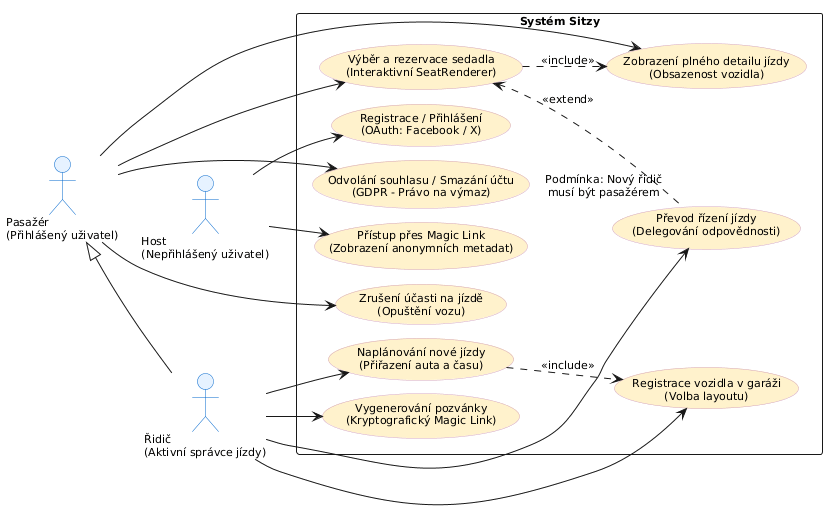
\includegraphics[width=0.9\linewidth]{images/01_usecase_v2.png}
\caption{UML diagram případů užití systému Sitzy}
\label{fig:usecase_diagram}
\zdroj{Vlastní zpracování v nástroji PlantUML.}
\end{figure}

Celkovou architekturu a technologické hranice systému zobrazuje komponentový diagram integrační architektury, který je dostupný v \extpriloha{externí příloze}{https://github.com/matthewjezek/thesis_ki_ujep/blob/fd77609d0333b87c656832fa3ce48e46de372957/images/16_component_diagram_v2.png}{komponentový diagram systému}. Diagram zachycuje zapojení primárních částí ekosystému a definuje toky dat a komunikační protokoly.

Volba této strategie a asynchronní komunikace přináší následující výhody:
\begin{enumerate}

\item \textbf{Ochrana klientských tajných klíčů (\textit{Client Secrets})}: Prostředí prohlížeče je z bezpečnostního hlediska považováno za veřejného klienta, což je nedůvěryhodné prostředí, kde nelze bezpečně uchovávat tajné klíče \cite{Denniss2017}. Pokud by se tajné klíče pro sociální sítě (např. \path{FACEBOOK_CLIENT_SECRET}) nacházely v klientské části, útočník by je mohl snadno extrahovat. Striktním oddělením vrstev jsou tyto údaje drženy výhradně na serveru v izolovaném prostředí backendu.

\item \textbf{Asynchronní model a škálovatelnost}: FastAPI je postaveno na asynchronním I/O modelu nad rozhraním ASGI. Využití tohoto modelu umožňuje aplikaci obsloužit vysoké množství souběžných integračních požadavků (např. OAuth callbacky) s minimální režií, což je klíčové pro minimalizaci latence při volání externích rozhraní sociálních sítí \cite{Mudassir20241030,FastAPI2026}.

\item \textbf{Nezávislost prezentační logiky}: Frontend se soustředí výhradně na vizualizaci a uživatelský zážitek (UX) pomocí komponent a specializovaných hooků \cite{React20251023}. Tím je zaručena plynulá interakce bez nutnosti opětovného přenačítání stránek.

\end{enumerate}

\section{Princip \UV{Security by Design} a bezheslová autentizace}

Bezpečnostní model \textit{Sitzy} plně implementuje princip \textit{Security by Design} a technické nařízení o~minimalizaci údajů podle nařízení GDPR tím, že zcela eliminuje lokální správu uživatelských hesel \cite{Naryama2026525,Cavoukian2010}. Odstraněním hesel je eliminován nejvýznamnější vektor útoku a riziko úniku přihlašovacích údajů (\textit{Credential Stuffing}) v případě narušení databáze.

Autentizace je plně delegována na prověřené poskytovatele identity splňující standardy OAuth 2.0 a OpenID Connect \cite{Hardt2012,Sakimura2023}. Zabezpečení SPA aplikací představuje z pohledu delegované autorizace komplexní problém. Specifikace RFC 9700 ukládá veřejným klientům povinnost implementovat mechanismus PKCE podle standardu RFC 7636 \cite{SakimuraEd2015, Lodderstedt2025}. Tento mechanismus chrání aplikaci před útoky na zachycení autorizačního kódu v nezabezpečeném prostředí prohlížeče \cite{SakimuraEd2015,Denniss2017}.

Proces bezpečného přihlášení s využitím PKCE a jednorázového stavového tokenu (\texttt{state}) jako ochrany proti CSRF útokům je znázorněn v \extpriloha{sekvenčním diagramu}{https://github.com/matthewjezek/thesis_ki_ujep/blob/fd77609d0333b87c656832fa3ce48e46de372957/images/12_sequence_delegated_auth_pkce.png}{sekvenční diagram bezheslové autentizace}. Diagram zachycuje jednotlivé kroky autorizačního toku od inicializace až po výměnu kódu na token, včetně kryptografického provázání pomocí PKCE.

Nakládání s tokeny na backendu a jejich životní cyklus odpovídá bezpečnostním doporučením NIST SP 800-204 \cite{Chandramouli2019} a osvědčeným architektonickým vzorům pro JWT relace \cite{Andrushchak202661}. Navržený model využívá dvouvrstvý systém:

\begin{itemize}

\item \textbf{Přístupový token}: Krátkodobý asynchronně verifikovatelný JWT token s platností 15~minut, odesílaný frontendu pro autorizaci běžných požadavků \cite{Jones2015,Andrushchak202661}.

\item \textbf{Obnovovací token}: Dlouhodobý stavový token s platností 7 dní, který je ukládán do databáze a přenášen v HTTP hlavičce jako zabezpečená cookie s příznaky \texttt{HttpOnly} (prevence XSS), \texttt{Secure} (vynucení HTTPS) a \texttt{SameSite=Lax} (prevence CSRF) \cite{Andrushchak202661,Rujichaikul20251014}.

\end{itemize}

\section{Relační datový model a správa relací}

Relační schéma v databázi PostgreSQL je navrženo ve třetí normální formě (3NF) s cílem zajistit datovou integritu a podporu pro asynchronní správu sezení z více zařízení současně \cite{Elmasri2016}. Struktura entit a jejich kardinality jsou zobrazeny v \extpriloha{entitně-relačním diagramu}{https://github.com/matthewjezek/thesis_ki_ujep/blob/fd77609d0333b87c656832fa3ce48e46de372957/images/13_erd_normalized.png}{normalizovaný entitně-relační diagram}.

Relační model se skládá z deseti entit:

\begin{enumerate}

\item \textbf{User (\texttt{users})}: Reprezentuje profil uživatele. Obsahuje unikátní identifikátor (UUID), jméno, e-mailovou adresu (označenou jako \textit{nullable}, neboť některé sítě e-mail neposkytují) a odkaz na profilový obrázek.

\item \textbf{SocialAccount (\path{social_accounts})}: Trvalé propojení uživatele s externími poskytovateli identity. Uchovává název poskytovatele, unikátní ID ze sociální sítě a vazbu na uživatelský profil.

\item \textbf{SocialSession (\path{social_sessions})}: Uchovává aktivní autorizační sezení uživatelů včetně hashovaného refresh tokenu a otisku klientského prohlížeče.

\item \textbf{Car (\texttt{cars})}: Reprezentuje vozidla vlastněná uživateli. Každé auto má definovaný typ uspořádání sedadel (\texttt{layout}) a vazbu na vlastníka v kardinalitě \texttt{1:N}.

\item \textbf{Seat (\texttt{seats})}: Reprezentuje jednotlivá sedadla. Existence sedadla je závislá na vozidle, což je vyjádřeno pomocí kompozitního primárního klíče \path{(car_id, position)}. Jde o~\textbf{identifikující vazbu} \cite{Elmasri2016}.

\item \textbf{CarDriver (\path{car_drivers})}: Uchovává historii přiřazení řidičů k vozidlům. Je vynuceno, že ke každému vozidlu v daném čase existuje právě jeden aktivní řidič.

\item \textbf{Ride (\texttt{rides})}: Reprezentuje naplánované jízdy včetně cíle, času odjezdu a kapacity.

\item \textbf{Passenger (\texttt{passengers})}: Spojovací tabulka pro obsazená sedadla během konkrétní jízdy. Reprezentuje vazbu mezi uživatelem, jízdou a konkrétním sedadlem.

\item \textbf{Invitation (\texttt{invitations})}: Ukládá vygenerované pozvánky. Obsahuje kryptografický token (32 bajtů), e-mail pozvaného a čas expirace.

\item \textbf{IntegrationAuditLog (\path{integration_audit_logs})}: Slouží k auditování klíčových integračních událostí a bezpečnostních změn v datovém formátu JSON.

\end{enumerate}

\subsection{Vzorec \UV{Dual Foreign Key} v tabulce SOCIAL\_SESSIONS}

Tento architektonický vzor řeší požadavek na striktní oddělení trvalé identity uživatele od dočasných autorizačních sezení \cite{Andrushchak202661}. Tradiční uložení tokenů přímo k profilu uživatele by omezilo přihlášení na jedno zařízení. Normalizací schématu a zavedením tabulky \path{SOCIAL_SESSIONS} je umožněn souběžný přístup z více zařízení. Tabulka využívá kompozitní vazbu pomocí dvou cizích klíčů: \path{user_id} (vazba na trvalou identitu) a \path{account_id} (vazba na konkrétní propojení se sítí). Zavedení sloupce \path{revoked_at} umožňuje okamžité zneplatnění konkrétní relace bez narušení celkového propojení uživatele se sociální sítí \cite{Rujichaikul20251014}.

\subsection{Programové vynucení GDPR mechanismů}
\label{sec:gdpr_mechanismy}

Návrh databázové struktury technicky vynucuje požadavky nařízení GDPR, konkrétně právo na výmaz (\textit{Right to be Forgotten}) podle Čl. 17 GDPR, přímo na úrovni databázového stroje pomocí referenční integrity \cite{Paisner25cervence2017,GDPR2016}:

\begin{itemize}

\item \textbf{Kaskádní odstraňování} (\texttt{ON DELETE CASCADE}): Při smazání uživatelského účtu databáze automaticky odstraní veškerá související sezení, propojené účty, vozidla a rezervace. Tím je zaručeno, že v systému nezůstanou žádná osiřelá osobní data \cite{Paisner25cervence2017}.

\item \textbf{Zachování auditní stopy} (\texttt{ON DELETE SET NULL}): Z bezpečnostních důvodů jsou veškeré záznamy v tabulce \path{INTEGRATION_AUDIT_LOGS} přísně chráněny před kaskádním smazáním. Při odstranění uživatele je cizí klíč nastaven na hodnotu \texttt{NULL}, čímž je zachována celistvost bezpečnostních logů bez uložení osobních identifikátorů.

\end{itemize}

\section{Distribuce pozvánek (Magic Links) jako řízení rizik API}

Během návrhu a vývoje distribuční vrstvy se v plné míře projevila tvrdá realita restrikcí korporátních ekosystémů, jejichž platformní a administrativní limity byly podrobně analyzovány a definovány v podkapitole \vref{subsec:od_otevrenych_protokolu_k_proprietarnim_rozhranim}. Velké platformy pod záminkou ochrany soukromí značně omezily svá aplikační rozhraní pro nezávislé vývojáře. Získání sociálního grafu přátel je dnes podmíněno složitým procesem schvalování (\textit{App Review}) a povinným firemním ověřením, což tvoří překážku pro akademické a studentské projekty \cite{DeNardis2015,MetaDeveloper20251030}.

Jako strategická architektonická reakce na identifikovaná omezení byl navržen decentralizovaný systém distribuce pozvánek prostřednictvím kryptografických jednorázových odkazů (tzv. \textit{Magic Links}). Tento autonomní distribuční kanál zcela obchází potřebu přímého přístupu k sociálnímu grafu uzavřených platforem, které v navrženém modelu figurují výhradně jako externí poskytovatelé identity, zatímco samotná koordinace a propojování komunity probíhá plně v režii aplikace \textit{Sitzy} nezávisle na platformních rozhraních \cite{MagicLinkIF}. V rámci tohoto procesu uživatel vygeneruje unikátní odkaz pro konkrétní jízdu a ten následně distribuuje skrze otevřené komunikační kanály, které jeho uzavřená komunita přirozeně využívá (např. Discord či Telegram).

Životní cyklus pozvánky, která slouží jako most pro bezpečný onboarding uživatelů, je znázorněn na stavovém diagramu na obrázku \vref{fig:invitation_lifecycle}.

\begin{figure}[htbp]
\centering
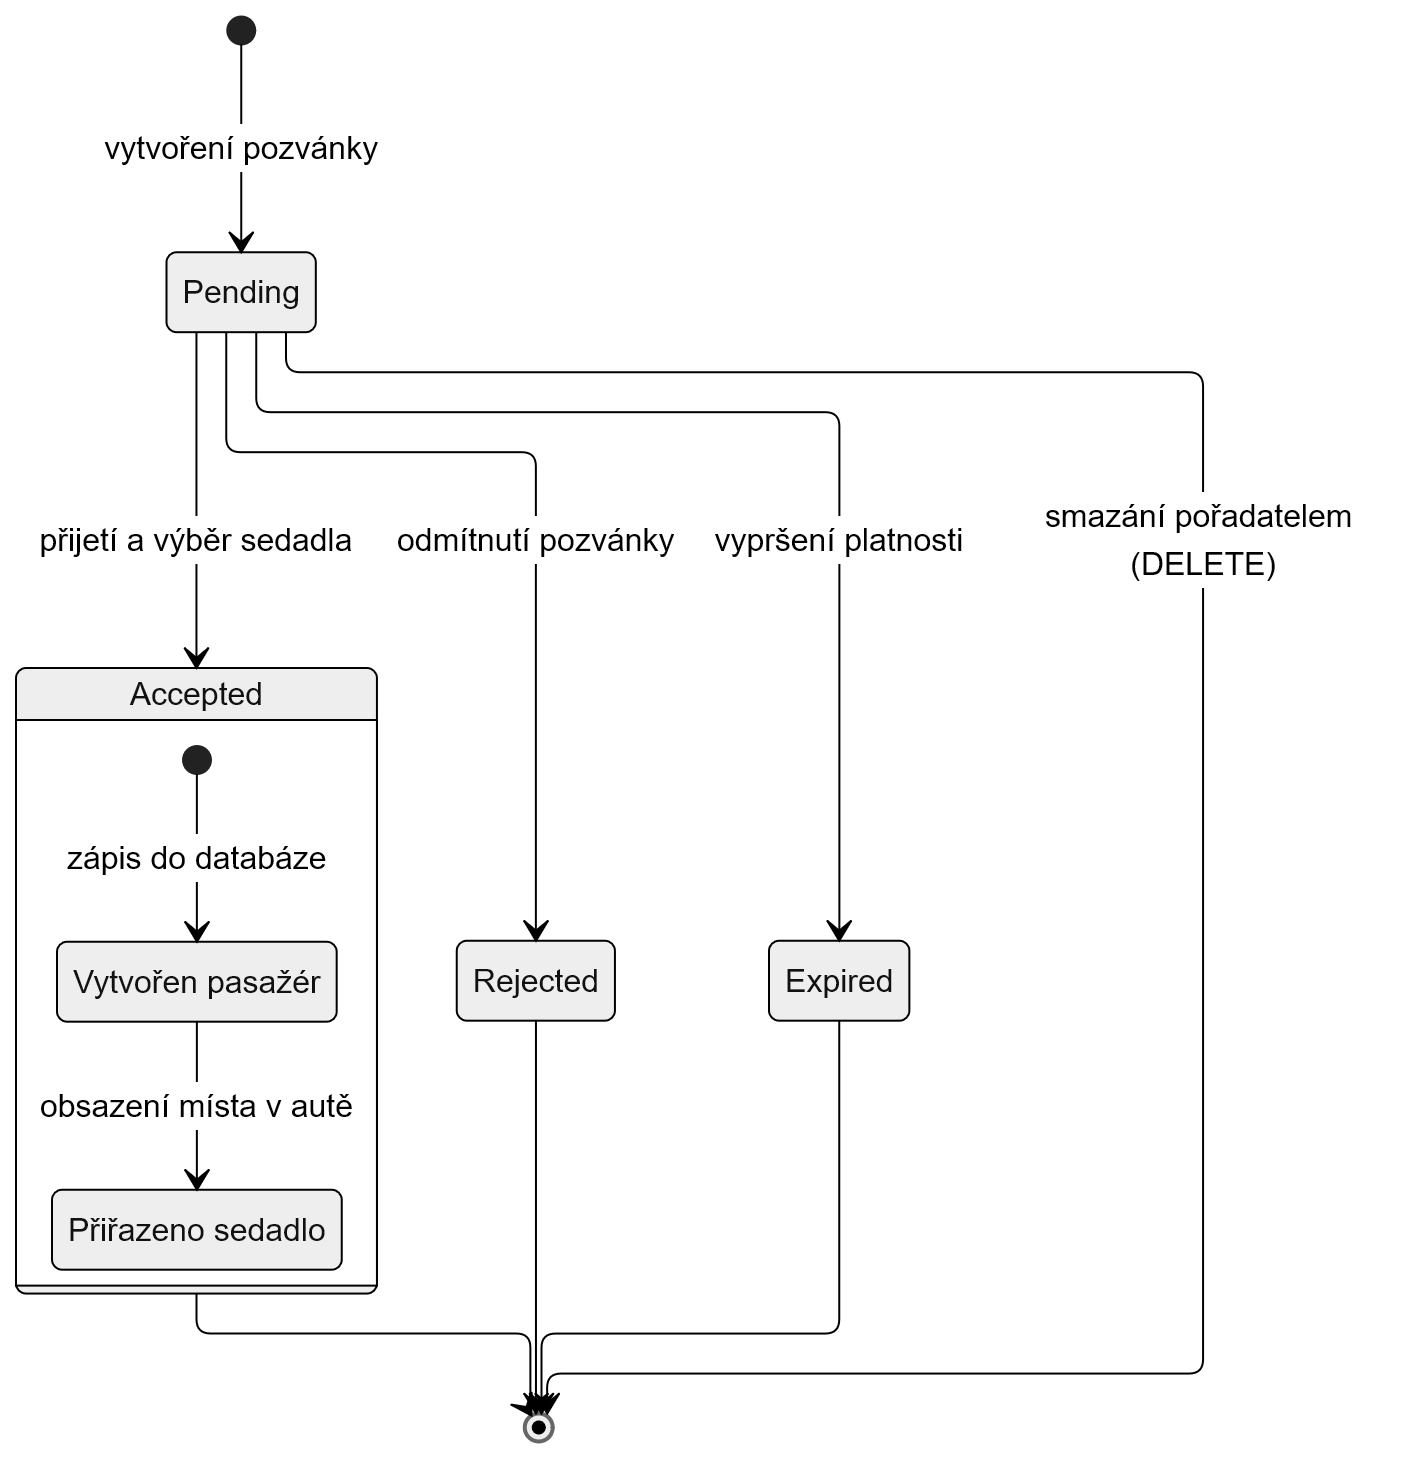
\includegraphics[width=0.8\linewidth]{images/06_state_invitation_lifecycle.png}
\caption{Stavový diagram životního cyklu pozvánky a účasti na jízdě}
\label{fig:invitation_lifecycle}
\zdroj{Vlastní zpracování v nástroji Mermaid.}
\end{figure}

Tento automat zaručuje onboarding bez ztráty kontextu a respektuje zásady ochrany soukromí:

\begin{enumerate}

\item \textbf{Uživatel (řidič)}: Naplánuje jízdu a vygeneruje unikátní odkaz s bezpečným 32bajtovým tokenem, který odešle do skupinového chatu.

\item \textbf{Host}: Klikne na odkaz. Klientská aplikace asynchronně zavolá veřejný endpoint, který validuje expiraci tokenu a načte metadata jízdy bez nutnosti okamžité registrace.

\item \textbf{Uložení kontextu}: Pokud host projeví zájem o místo, frontend dočasně uloží token do \texttt{sessionStorage} a přesměruje jej na OAuth přihlášení IdP.

\item \textbf{Spárování}: Po úspěšném přihlášení frontend detekuje token v \texttt{sessionStorage} a asynchronně odešle požadavek na přijetí pozvánky. Backend automaticky spáruje novou federovanou identitu s pozvánkou a zapíše záznam do tabulky \texttt{PASSENGERS}. Tento postup plně vyhovuje rámci deidentifikace a ochrany dat podle GDPR \cite{Paisner25cervence2017}.

\end{enumerate}

\chapter{Realizace a nasazení systému}
\label{chap:realizace_qa_nasazeni}

Tato kapitola je věnována detailnímu rozboru praktické realizace, technologické implementace, zajištění kvality a produkčního nasazení referenční webové platformy \textit{Sitzy}. Cílem textu je demonstrovat, jak byly principy softwarové modularity, asynchronního zpracování dat, delegované federované identity a přísného zabezpečení transformovány do reálné programové báze. Vývoj celého systému probíhal s důrazem na typovou bezpečnost, modularitu kódu a odolnost vůči platformním rizikům a omezením korporátních ekosystémů.

\section{Portálová registrace a konfigurace integračních rozhraní}
\label{sec:portalova_registrace}

Před zahájením samotné implementace klientské i serverové části bylo nutné provést registraci a~konfiguraci aplikací v partnerských vývojářských konzolích poskytovatelů identit. Tento proces ustavuje společnou konfigurační bázi, která je nezbytná pro bezpečné propojení lokálního prostředí (a později i produkčního) s externími autorizačními servery.

\subsection{Společná konfigurační báze a správa identifikačních klíčů}
\label{subsec:spolecna_konfiguracni_baze_a_sprava_identifikacnich_klicu}

Prostředí lokálního repozitáře se opírá o environmentální izolaci citlivých parametrů, což je popsáno později v podkapitole \vref{sec:technologicka_modularita}. Jedinečné identifikátory \path{CLIENT_ID} (případně \path{App ID} u sítě Facebook) a tajné klíče \path{CLIENT_SECRET} jsou získávány z jednotlivých vývojářských portálů a ukládány do lokálního konfiguračního souboru \path{.env}, který je vyloučen z verzování.

Důležitým bezpečnostním krokem v souladu s doporučením standardu RFC 9700 \cite{Lodderstedt2025} je definice striktních Redirect URIs. Autorizační servery vyžadují exaktní porovnávání řetězců, což zamezuje exfiltraci autorizačních kódů. V rámci implementace bylo nutné definovat odlišné parametry pro jednotlivá běhová prostředí. Zatímco lokální vývojový server je provozován na portu 5173 s~adresou \path{http://localhost:5173/auth/callback}, pro ostré produkční nasazení byla zvolena zabezpečená doména \path{https://sitzy.page}. Určitou výjimkou je zde platforma Facebook, která při vývoji aplikace automaticky přijímá komunikaci z lokálních prostředí bez nutnosti fyzického zapsání těchto URL do seznamu povolených URI.

\subsection{Konfigurace v rozhraní Meta for Developers}

Registrace aplikace v portálu Meta vyžaduje výběr dedikovaného scénáře použití \UV{Authenticate and request data from users with Facebook Login}, jak je znázorněno v \extpriloha{externí příloze}{https://github.com/matthewjezek/thesis_ki_ujep/blob/fd77609d0333b87c656832fa3ce48e46de372957/images/meta_app_use_cases.png}{výřez z Meta for Developers (Use case)}. 

Z hlediska legislativního souladu s nařízením GDPR byla v nastavení produktu Facebook Login nakonfigurována adresa pro zpracování požadavků na odstranění dat (\textit{User Data Deletion Callback URL}), která odkazuje na chráněný asynchronní endpoint \path{/auth/facebook/deletion} popsaný v~podkapitole \vref{sec:gdpr_compliance}. Podrobnosti konfigurace jsou dostupné v \extpriloha{externí příloze}{https://github.com/matthewjezek/thesis_ki_ujep/blob/fd77609d0333b87c656832fa3ce48e46de372957/images/meta_app_basic_settings.png}{výřez z Meta for Developers (Basic settings)}.

Vzhledem k výzkumnému charakteru práce a absenci firemního ověření (\textit{Business Verification}) běží aplikace v režimu vývoje. Jak bylo rozebráno v části \vref{subsec:sprava_uzivatelskych_roli_v_testovacim_rezimu}, role \UV{Consumer Tester} v reálném uživatelském rozhraní Meta neexistuje navzdory její deklaraci v oficiální dokumentaci. Testování bylo proto realizováno manuálním přidáváním uživatelů do role \path{Tester} v sekci \UV{App Roles}, což vyžaduje, aby všechny testující subjekty vlastnily registrovaný vývojářský účet. Vizuální dokumentace tohoto procesu je dostupná v \extpriloha{externí příloze}{https://github.com/matthewjezek/thesis_ki_ujep/blob/fd77609d0333b87c656832fa3ce48e46de372957/images/meta_app_roles.png}{výřez z Meta for Developers (Roles)}. Tato situace potvrzuje dokumentační dluh platformy a zvyšuje technologickou bariéru pro nezávislé vývojáře.

\subsection{Konfigurace v prostředí X Developer Console}

Proces založení aplikace v portálu X Developer Console se vyznačuje odlišným přístupem. Po~vytvoření aplikace jsou vývojáři jednorázově zobrazeni kritické přístupové klíče (\texttt{Consumer Key}, \texttt{Secret Key}, \texttt{Bearer Token}), které nelze později opětovně zobrazit a musí být okamžitě zapsány do konfiguračního souboru \path{.env}. Podrobnosti tohoto procesu jsou dokumentovány v \extpriloha{externí příloze}{https://github.com/matthewjezek/thesis_ki_ujep/blob/fd77609d0333b87c656832fa3ce48e46de372957/images/x_app_credentials.png}{výřez z X Developer Console (Credentials)}.

Aktivace protokolu OAuth 2.0 vyžaduje specifickou konfiguraci v sekci \textit{Authentication settings}. Volbou typu aplikace \textit{Web App, Automated App or Bot} je systém Sitzy definován jako \textit{confidential client}, což umožňuje bezpečnou izolaci \textit{client secret} na backendu. Vizualizace tohoto nastavení je dostupná v \extpriloha{externí příloze}{https://github.com/matthewjezek/thesis_ki_ujep/blob/fd77609d0333b87c656832fa3ce48e46de372957/images/x_app_type.png}{výřez z X Developer Console (App type)}.

V sekci \textit{App info} byly specifikovány povinné parametry \textit{Callback URI} a \textit{Website URL}. Podrobnosti jsou dostupné v \extpriloha{externí příloze}{https://github.com/matthewjezek/thesis_ki_ujep/blob/fd77609d0333b87c656832fa3ce48e46de372957/images/x_app_info.png}{výřez z X Developer Console (App info)}.

Rozsah oprávnění byl v souladu se zásadou minimalizace dat omezen na úroveň \textit{Read}, která postačuje k získání unikátního identifikátoru a základních profilových údajů. Pro přístup k~e-mailové adrese skrze scope \path{users.email} bylo nutné aktivovat volbu \UV{Request email from users}, která podmiňuje funkčnost integrace uvedením validních odkazů na zásady ochrany soukromí a~smluvní podmínky. Tato administrativa přináší pro nezávislé projekty povinnost vytvoření právního rámce již v rané fázi vývoje. Konfigurace oprávnění je zobrazena v \extpriloha{externí příloze}{https://github.com/matthewjezek/thesis_ki_ujep/blob/fd77609d0333b87c656832fa3ce48e46de372957/images/x_app_permissions.png}{výřez z X Developer Console (App permissions)}.

\section{Technologická modularita a monorepo platformy}
\label{sec:technologicka_modularita}

\subsection{Struktura a koncové body autentizačního modulu} \label{subsec:prehled_routeru_auth}

Jádrem integrační logiky je router \path{auth.py}, který definuje rozhraní pro správu federované identity a řízení relací. Propojení teoretického návrhu z kapitoly 4 s praktickou realizací zajišťuje datový model \texttt{SocialSession}. Tento model implementuje vzor Dual-FK (viz ukázka \vref{lst:social_session_model}), čímž ustavuje pevnou vazbu mezi konkrétní relací, identitou uživatele a zdrojovým sociálním účtem.

\begin{listing}[htbp]
\begin{minted}[
    frame=lines,
    framesep=2mm,
    baselinestretch=1.1,
    fontsize=\footnotesize,
    linenos=false
]{python}
class SocialSession(Base):
    __tablename__ = "social_sessions"
 
    id: Mapped[uuid.UUID] = mapped_column(
        PG_UUID(as_uuid=True), primary_key=True, default=uuid.uuid4
    )
    user_id: Mapped[uuid.UUID] = mapped_column(
        PG_UUID(as_uuid=True), ForeignKey("users.id"), nullable=False, index=True
    )
    social_account_id: Mapped[uuid.UUID] = mapped_column(
        PG_UUID(as_uuid=True),
        ForeignKey("social_accounts.id"),
        nullable=False,
        index=True,
    )
    access_token: Mapped[str] = mapped_column(String, nullable=False)
    refresh_token: Mapped[str | None] = mapped_column(String, nullable=True)
    expires_at: Mapped[datetime] = mapped_column(
        DateTime(timezone=True), nullable=False, index=True
    )
    user_agent: Mapped[str | None] = mapped_column(String, nullable=True)
    created_at: Mapped[datetime] = mapped_column(
        DateTime(timezone=True), nullable=False, server_default=text("now()")
    )
    revoked_at: Mapped[datetime | None] = mapped_column(
        DateTime(timezone=True), nullable=True, index=True
    )
 
    user: Mapped["User"] = relationship(back_populates="social_sessions")
    social_account: Mapped["SocialAccount"] = relationship(back_populates="sessions")
\end{minted}
\caption{Implementace modelu SocialSession podporující Dual-FK vazbu}
\label{lst:social_session_model}
\zdroj{Vlastní zpracování v rámci vývoje backendu.}
\end{listing}

Funkcionalita modulu je distribuována skrze následující koncové body:
 
\begin{itemize}
\item \path{/oauth/facebook/init} a \path{/oauth/x/init}: Dvojice
provider-specifických endpointů, které inicializují OAuth tok vygenerováním
unikátního stavu a přesměrováním uživatele na autorizační server
příslušného poskytovatele.
 
\item \path{/oauth/callback}: Zpracovává návratový požadavek z externí sítě,
provádí výměnu autorizačního kódu za tokeny a ustavuje lokální relaci.
 
\item \path{/refresh}: Zajišťuje kontinuitu přihlášení vydáním nového
přístupového tokenu na základě validní \texttt{HttpOnly} cookie.
 
\item \path{/revoke}: Okamžitě zneplatňuje aktuální relaci v databázi i
v klientském prohlížeči.
 
\item \path{/me}: Navrací normalizované profilové údaje aktuálně
autentizovaného uživatele pro potřeby frontendu.
 
\item \path{/social/dashboard}: Agreguje přehled připojených účtů, historii
integračních událostí a~seznam aktivních zařízení.
 
\item \path{/social/sessions/{session_id}/revoke}: Umožňuje zneplatnit
konkrétní relaci podle jejího identifikátoru, například ze seznamu aktivních
zařízení v dashboardu.
 
\item \path{/social/sessions/revoke-others}: Bezpečnostní funkce umožňující
hromadné ukončení všech ostatních relací daného uživatele s výjimkou té
aktuální.
 
\item \path{/social/providers/{provider}/unlink}: Odpojuje konkrétního
poskytovatele identity od uživatelského účtu; operace je blokována, pokud by
šlo o posledního zbývajícího poskytovatele nebo o poskytovatele, jehož
relací je uživatel právě přihlášen.
 
\item \path{/delete-account}: Realizuje proces kompletní anonymizace a
odstranění uživatelských dat v souladu s mechanismy popsanými v sekci
\vref{sec:gdpr_compliance}.
 
\item \path{/facebook/deletion}: Specializovaný webhook vyžadovaný
platformou Meta pro asynchronní potvrzení požadavků na výmaz dat.
 
\item \path{/users/{user_id}/avatar}: Inteligentní proxy endpoint, který
dynamicky obnovuje expirované odkazy na profilové obrázky ze sítě Facebook.
\end{itemize}

Projekt je strukturován jako monorepo, což umožňuje centralizovanou správu klientské i serverové části v jednom verzovacím prostoru a definování jednotných pravidel pro statickou analýzu, formátování kódu a testovací scénáře. Toto uspořádání výrazně usnadňuje synchronizaci datových schémat a garantuje, že klientská část pracuje s identickými datovými kontrakty jako serverový backend.

Fyzická struktura repozitáře a logické rozdělení odpovědností jsou znázorněny v následujícím hierarchickém schématu. Zdrojový kód aplikace je dostupný v repozitáři, na který odkazuje příloha \vref{sec:ep}.
 
\begin{minipage}{\linewidth}
\dirtree{%
.1 Sitzy/ .
.2 api/ \quad $\leftarrow$ Zdrojový kód serverového backendu (FastAPI).
.3 core/ \quad $\leftarrow$ Globální konfigurace, logger a rate limiter.
.3 routers/ \quad $\leftarrow$ API směrovače (auth, cars, invitations, rides).
.3 services/ \quad $\leftarrow$ Aplikační služby (oauth\_service.py).
.3 models.py \quad $\leftarrow$ SQLAlchemy databázové modely.
.3 schemas.py \quad $\leftarrow$ Pydantic validační a serializační schémata.
.2 frontend/ \quad $\leftarrow$ Zdrojový kód klientské aplikace (React).
.3 src/.
.4 components/ \quad $\leftarrow$ Znovupoužitelné UI komponenty.
.4 hooks/ \quad $\leftarrow$ Vlastní React hooky (useAuth, useInvites).
.4 pages/ \quad $\leftarrow$ Komponenty stránek (OAuthCallbackPage).
.4 types/ \quad $\leftarrow$ Deklarace sdílených TypeScript typů (models.ts).
.4 api/ \quad $\leftarrow$ Konfigurace Axios klienta a interceptorů.
.3 public/ \quad $\leftarrow$ Statické veřejné dokumenty.
.3 vite.config.ts \quad $\leftarrow$ Konfigurační skript pro Vite.
.2 alembic/ \quad $\leftarrow$ Skripty a verze databázových migrací.
.2 docker-compose.yml \quad $\leftarrow$ Orchestrace PostgreSQL a Redis v Dockeru.
.2 .env \quad $\leftarrow$ Konfigurace prostředí.
}
\end{minipage}
\label{struktura_repozitare}

\subsection{Asynchronní backend (FastAPI a SQLAlchemy)}

Volba asynchronního frameworku FastAPI na backendu byla určena požadavkem na vysokou propustnost a nízkou latenci při zpracování vícenásobných síťových volání směrem k externím API sociálních sítí (výměna autorizačních kódů, dotazy na profilová data). Ve srovnání s tradičními synchronními frameworky umožňuje asynchronní model, využívající rozhraní ASGI, efektivní zpracování I/O operací bez blokování operačního vlákna. To je klíčové, protože komunikace s~externími poskytovateli identity představuje nejvýraznější latenční úzké hrdlo celého systému.

Relační perzistence je zajištěna objektově-relačním mapováním pomocí SQLAlchemy, které přináší plnou typovou podporu prostřednictvím konstruktů \texttt{Mapped} a deklarativního mapování. SQL~dotazy jsou tak již ve fázi vývoje typově kontrolovány nástrojem \texttt{mypy} v nejstriktnějším režimu, což eliminuje běhové chyby pramenící z nekonzistentních datových typů.

\subsection{Typově bezpečný frontend (React a TypeScript)}

Klientská Single Page aplikace je implementována v knihovně React s plným využitím statického typování v jazyce TypeScript. Klientský stav a směrování jsou řízeny knihovnou React Router, která nativně podporuje asynchronní načítání komponent a zapouzdření chráněných cest. 

Pro zachování absolutní integrity API kontraktů a zamezení ručnímu přepisování typů při každé změně na backendu byla zavedena strategie zrcadlení datových schémat. Typové definice v~klientském souboru \path{frontend/src/types/models.ts} jsou striktně odvozeny a typově mapovány podle validačních a serializačních schémat Pydantic, které definuje backend v souboru \path{api/schemas.py}. Při jakékoliv změně v databázové struktuře nebo API kontraktu na backendu tak dojde k okamžitému zachycení nekonzistence při statické kompilaci frontendu. Vzhled a~stylizace klientského rozhraní jsou postaveny na utility-first CSS frameworku Tailwind CSS, který díky Rust kompilátoru zajišťuje okamžitý build a minimalizaci výsledného CSS bundle.

\subsection{Bezpečné řízení relací a asynchronní správa stavu}
\label{sec:rizeni_relaci}

Během implementace bezheslového toku a integrace sítě X se jako nezbytné ukázalo bezpečné a dočasné ukládání jednorázových stavových kódů (\path{state}) a PKCE verifikátorů na backendu. Pro tyto účely bylo zvoleno rychlé in-memory úložiště Redis, které umožňuje definovat časovou expiraci klíčů. Aby se spolehlivě zabránilo útokům typu opakovaného použití tokenů (\textit{Replay Attacks}), byla pro ověření stavu implementována atomická operace \texttt{getdel}, která v jediném kroku hodnotu vyhledá a okamžitě z paměti smaže.

Ověření stavu OAuth pomocí atomické operace v kódové bázi je implementováno v následující ukázce funkce \vref{lst:redis_getdel}:

\begin{listing}[htbp]
\begin{minted}[
    frame=lines,
    framesep=2mm,
    baselinestretch=1.1,
    fontsize=\footnotesize,
    linenos=false
]{python}
def validate_and_consume_state(
    self, state: str
) -> tuple[Provider, str | None] | None:
    raw = _redis.getdel(self._key(state))
    if not raw:
        logger.warning("OAuth state validation failed - state not found")
        return None
    data = json.loads(raw)
    logger.debug(
        "OAuth state validated and consumed",
        extra={"provider": data.get("provider")},
    )
    return data["provider"], data.get("code_verifier")
\end{minted}
\caption{Ověření a konzumace jednorázového stavu OAuth v paměti Redis}
\label{lst:redis_getdel}
\zdroj{Vlastní zpracování v rámci vývoje pilotního systému.}
\end{listing}

Další významná technická překážka se projevila při nasazení aplikace do produkčního prostředí na chráněné doméně \path{https://sitzy.page}. Bezpečnostní politiky moderních webových prohlížečů na ochranu soukromí (zejména Apple Safari Intelligent Tracking Prevention) za určitých podmínek blokují ukládání a přenos \textit{host-only} cookies, pokud jsou nastaveny z odlišné subdomény (např. z~asynchronního API běžícího na \path{api.sitzy.page}).

Tato komplikace byla vyřešena na úrovni backendu úpravou zápisu cookies. Při úspěšném přihlášení je dlouhodobý obnovovací token (\path{refresh_token}) zapsán jako \path{HttpOnly} a \path{Secure} cookie s příznakem \path{SameSite=Lax}. Klíčovým krokem však byla explicitní konfigurace cesty na kořen (\path{path="/"}) a dynamické parsování domény z nastavení frontendového původu pro zafixování na hlavní doménu druhé úrovně (např. \path{domain=".sitzy.page"}), což prohlížeči explicitně povoluje sdílení cookie napříč všemi subdoménami.

Nastavení a zápis zabezpečené cookie pro root doménu je uvedeno v následující ukázce funkce:

\begin{listing}[htbp]
\begin{minted}[
    frame=lines,
    framesep=2mm,
    baselinestretch=1.1,
    fontsize=\footnotesize,
    linenos=false
]{python}
def _set_refresh_cookie(response: Response, refresh_token: str) -> None:
    from urllib.parse import urlparse

    domain: str | None = None
    if settings.environment == "production":
        parsed_url = urlparse(settings.frontend_origin)
        hostname = parsed_url.hostname
        if hostname:
            parts = hostname.split(".")
            if len(parts) >= 2:
                domain = ".".join(parts[-2:])

    response.set_cookie(
        key="refresh_token",
        value=refresh_token,
        httponly=True,
        secure=settings.environment == "production",
        samesite="lax",
        max_age=settings.refresh_token_expire_days * 24 * 3600,
        path="/",
        domain=domain,
    )
\end{minted}
\caption{Konfigurace a zápis HttpOnly cookie s dynamickou doménovou fixací}
\label{lst:set_cookie}
\zdroj{Vlastní zpracování v rámci vývoje pilotního systému.}
\end{listing}

\section{Technické ošetření compliance a GDPR mechanismů}
\label{sec:gdpr_compliance}

Zatímco referenční integrita a kaskádní pravidla na úrovni databázového schématu, popsaná v sekci \vref{sec:gdpr_mechanismy}, zajišťují spolehlivou fyzickou likvidaci osobních údajů přímo v relační struktuře PostgreSQL, v aplikační vrstvě bylo nutné implementovat robustní prováděcí cestu. Vynucení práva na výmaz podle Článku 17 nařízení GDPR \cite{GDPR2016} je programově realizováno na asynchronním backendu prostřednictvím chráněného koncového bodu \path{DELETE /auth/delete-account}. Tento endpoint je zpřístupněn pouze autentizovaným uživatelům po úspěšném ověření jejich identity, přičemž je chráněn aplikačním omezovačem požadavků s frekvencí limitovanou na tři volání za minutu za účelem mitigace útoků typu DoS (\textit{Denial of Service}). Při jeho vyvolání asynchronní služba provede smazání uživatelského objektu v rámci databázové relace SQLAlchemy, což automaticky spouští kaskádní odstraňování dat, a současně vyvolá explicitní revokaci aktivních tokenů v~in-memory cache Redis a vyčištění klientské \texttt{HttpOnly} cookie.

Mimo interní vyvolání smazání vyžadují zásady platformy Meta pro produkční provoz federovaného přihlašování integraci asynchronního webhooku pro zpětné volání (\textit{Facebook Data Deletion Request Callback}) na veřejném endpointu \path{POST /auth/facebook/deletion}. Tento endpoint zpracovává podepsaný požadavek \path{signed_request} předávaný ve formě POST formuláře. Z~důvodu ochrany proti podvržení dat nebo útokům založeným na analýze délky zpracování požadavků (\textit{Timing Attacks}) je nezbytné provést striktní kryptografické ověření digitálního podpisu zaslaného payloadu s využitím tajného klíče aplikace (\path{facebook_client_secret}). Absence tohoto ověření by endpoint vystavila riziku podvržené autentizace \cite{Yalon2023API2}.

Formát \path{signed_request} se skládá z hlavičky a payloadu oddělených tečkou, přičemž obě části jsou kódovány v base64url bez zarovnávacích znaků a podpis je vytvořen algoritmem HMAC-SHA256 s využitím tajného klíče aplikace. Ukázka bezpečného parsování, doplnění chybějícího Base64 zarovnání a verifikace HMAC-SHA256 podpisu je uvedena v následujícím kódu \vref{lst:fb_signature_verify}:

\begin{listing}[htbp]
\begin{minted}[
    frame=lines,
    framesep=2mm,
    baselinestretch=1.1,
    fontsize=\footnotesize,
    linenos=false
]{python}
@router.post("/facebook/deletion", status_code=status.HTTP_200_OK)
@limiter.limit("10/minute")
def facebook_data_deletion_callback(
    signed_request: str = Form(...), db: Session = Depends(get_db)
) -> dict[str, str]:
    encoded_sig, payload = signed_request.split(".", 1)
    decoded_sig = base64.urlsafe_b64decode(_pad(encoded_sig))

    expected_sig = hmac.new(
        settings.facebook_client_secret.encode("utf-8"),
        msg=payload.encode("utf-8"),
        digestmod=hashlib.sha256,
    ).digest()

    if not hmac.compare_digest(decoded_sig, expected_sig):
        raise ValueError("Signature verification failed")

    data = json.loads(base64.urlsafe_b64decode(_pad(payload)))
    # ... zpracování data["user_id"] a smazání účtu
\end{minted}
\caption{Kryptografické ověření a dekódování callbacku signed\_request od sítě Facebook}
\label{lst:fb_signature_verify}
\zdroj{Vlastní zpracování v rámci vývoje pilotního systému.}
\end{listing}

Všechny citlivé endpointy autentizačního toku (inicializace OAuth, callback, obnova a odvolání tokenu, smazání účtu i deletion webhook) jsou opatřeny aplikačním omezovačem požadavků s~limity v rozmezí 3--30 volání za minutu, což mitiguje rizika neomezené spotřeby zdrojů (\textit{Unrestricted Resource Consumption}) \cite{Yalon2023API4}.

\section{Klientská optimalizace a ošetření chyb v mobilních prohlížečích} \label{sec:klientske_optimalizace}

Při návrhu a provozování klientské aplikace na platformě Heroku bylo nutné zohlednit finanční a~provozní limity infrastruktury. Z důvodu úspory systémových prostředků a zamezení vyčerpání provozního kreditu (které by vedlo k dodatečnému zpoplatnění vývoje mimo studentské tarify) bylo rozhodnuto upustit od pravidelné periodické aktualizace dat na pozadí pomocí klientského pollingu. Pravidelné asynchronní dotazování by totiž udržovalo Heroku dyno v trvale aktivním stavu a bránilo jeho přirozenému uspání v období neaktivity, což by vedlo k rychlému vyčerpání limitů a nechtěným nákladům.

Namísto pravidelných aktualizací se tak data obnovují až přirozeným navigováním uživatele napříč aplikací nebo při interagování s prvky jako jsou třeba oznámení. Vzhledem k charakteru aplikace správy jízd, které se plánují řádově na hodiny či dny dopředu, se toto řešení jeví jako dostačující a zároveň šetrné k provozním nákladům.

\subsection{Ošetření chyb v mobilních prohlížečích bez JIT kompilace}

Během externího testování na mobilních zařízeních byla odhalena specifická chybová anomálie u~uživatelů využívajících platformy se zvýšenou ochranou soukromí. Konkrétně se jednalo o~mobilní telefon Pixel s operačním systémem GrapheneOS a výchozím prohlížečem Vanadium (který reprezentuje privacy-first Chromium fork). Tento prohlížeč má z bezpečnostních důvodů ve výchozím nastavení zcela deaktivovanou JIT (\textit{Just-In-Time}) kompilaci JavaScriptu.

Deaktivace JIT kompilace sice výrazně zvyšuje odolnost proti zneužití paměťových zranitelností na úrovni klientského sandboxu, avšak spouští klientský kód v interpretačním režimu, který je však řádově pomalejší. V důsledku tohoto zpomalení docházelo během zpracování callbacku k~\textit{race condition}, kdy pomalý klientský prohlížeč odeslal na backend dva identické požadavky na ověření OAuth kódu v rozmezí několika desítek milisekund.

Jelikož backend v souladu se standardy striktně uplatňuje jednorázovost stavových tokenů a po prvním přečtení klíč z paměti Redis okamžitě maže (viz atomická operace \path{getdel} v ukázce kódu \vref{lst:redis_getdel}), první z těchto požadavků uspěl, avšak druhý okamžitě narazil na již neexistující stav a vrátil HTTP chybu \texttt{400 Bad Request}. Tato chybová odpověď následně na klientovi přepsala stav úspěšného přihlášení a uživatele přesměrovala zpět na přihlašovací obrazovku.

Tato kritická race condition byla na frontendu vyřešena implementací návrhového vzoru \textit{Singleton Promise Coalescing}~\cite{Andrushchak202661}. Klientská aplikace využívá globální modulovou mapu běžících asynchronních promisů, které stojí zcela mimo životní cyklus React komponenty. Pokud se stránka v důsledku pomalého interpretu nebo Strict Mode namontuje podruhé, nový síťový dotaz se již neodesílá, ale klientský kód se bezpečně napojí na již běžící asynchronní promise.

Tato klientská ochrana race condition je implementována následovně:

\begin{listing}[htbp]
\begin{minted}[
    frame=lines,
    framesep=2mm,
    baselinestretch=1.1,
    fontsize=\footnotesize,
    linenos=false
]{typescript}
const pendingCallbacks = new Map<string, Promise<{ access_token: string }>>()

export default function OAuthCallbackPage() {
  const [searchParams] = useSearchParams()
  const navigate = useNavigate()
  const code = searchParams.get('code')
  const state = searchParams.get('state')

  const [animationDone, setAnimationDone] = useState(!!navigator.webdriver)
  const [targetPath, setTargetPath] = useState<string | null>(null)

  useEffect(() => {
    if (!code || !state) {
      toast.error('Neplatný callback.')
      setTargetPath('/login')
      return
    }

    let promise = pendingCallbacks.get(state)
    if (!promise) {
      promise = instance.get('/auth/oauth/callback', { 
        params: { code, state }
      }).then(response => response.data)
      pendingCallbacks.set(state, promise)
    }

    let active = true

    promise
      .then(async data => {
        pendingCallbacks.delete(state)
        if (!active) return
        // ... uspesne zpracovani a prirazeni tokenu ...
\end{minted}
\caption{Ochrana race condition pomocí Singleton Promise Coalescing}
\label{lst:promise_coalescing}
\zdroj{Vlastní zpracování v rámci vývoje pilotního systému.}
\end{listing}

\subsection{Zachování kanonické domény při generování Open Graph metadat}
\label{sec:og_canonical_domain}

Distribuce odkazů vedoucích na dynamicky generovaný obsah (např. formulář uživatelského 
výzkumu na trase \path{/survey}) probíhá skrze bránu implementovanou jako Cloudflare 
Worker \cite{CloudflareDocsWorkers}, která funguje jako reverzní proxy a předává požadavky na statický frontend hostovaný na Vercelu a vynucuje autorizační hlavičku \path{x-worker-secret} mezi oběma vrstvami. Middleware zodpovědný za injektáž Open Graph meta tagů však chybně odvozoval hodnotu \path{og:url} z lokálního \path{url.origin} požadavku namísto veřejné domény \path{https://sitzy.page}. Při procházení odkazu crawlerem sociální sítě tak byla cílová URL sdíleného náhledu přepsána na interní adresu Vercelu, jak dokládá srovnání obou stavů \extpriloha{odkazu}{https://github.com/matthewjezek/thesis_ki_ujep/blob/7ad5c94cc4b78a01c40631bd5ae1d275058689d9/images/survey_link_difference.png}{porovnání různých vzhledů odkazu}. Uživatelé, kteří kliknutím na sdílenou pozvánku navigovali přímo na tuto interní adresu, obcházeli bránu i její autorizační hlavičku, což vedlo k chybě \texttt{403 Forbidden}. Náprava spočívala v explicitním vynucení veřejné domény při generování \path{og:url} nezávisle na tom, odkud middleware požadavek fyzicky obsluhuje.

\section{Normalizace federovaných uživatelských profilů}
\label{sec:normalizace_profilu}

Při integraci profilových obrázků poskytovaných externími poskytovateli identity bylo nutné vyřešit dva inženýrské problémy. Prvním je výskyt nešifrovaných (HTTP) nebo bezprotokolových odkazů, které na produkčním prostředí běžícím na HTTPS způsobují v prohlížečích chyby typu \textit{Mixed Content}. Druhým je omezená platnost podepsaných URL u sítě Facebook (standardně 24~hodin), což po expiraci vede k zobrazení nefunkčních odkazů (chyba HTTP 404).

Tento stav byl vyřešen implementací lokálního reverzního proxy serveru na backendu. V souboru \path{api/schemas.py} je integrována pomocná funkce \path{get_facebook_proxy_url}, která adresy obsahující domény \path{fbsbx.com} nebo \path{facebook.com} automaticky přepisuje na interní trasu \path{/auth/users/{user_id}/avatar}. K tomu je využit dekorátor \path{@model_validator(mode="after")} nad validačními schématy \path{UserOut}, \path{UserBasicOut} a \path{PassengerOut}, jak je demonstrováno ve výpisu \vref{lst:pydantic_avatar_proxy}.

\begin{listing}[htbp]
\begin{minted}[
    frame=lines,
    framesep=2mm,
    baselinestretch=1.1,
    fontsize=\footnotesize,
    linenos=false
]{python}
def get_facebook_proxy_url(user_id: UUID, current_avatar_url: str | None) -> str | None:
    if current_avatar_url and (
        "fbsbx.com" in current_avatar_url or "facebook.com" in current_avatar_url
    ):
        from urllib.parse import urlparse

        from api.config import settings

        parsed = urlparse(str(settings.facebook_redirect_uri))
        base_url = f"{parsed.scheme}://{parsed.netloc}"
        return f"{base_url}/auth/users/{user_id}/avatar"
    return current_avatar_url
\end{minted}
\caption{Pomocná funkce pro přepisování Facebook URL na lokální proxy}
\label{lst:pydantic_avatar_proxy}
\zdroj{Vlastní zpracování v rámci vývoje backendu.}
\end{listing}

Cílová adresa serverového požadavku na Facebook Graph API je v kódu zapsána staticky (\path{graph.facebook.com}) a není odvozena z uživatelského vstupu, čímž je eliminováno riziko Server-Side Request Forgery \cite{Yalon2023API7}, které by jinak hrozilo při dynamickém sestavování cílové URL serverového požadavku.

Samotné odbavení a směrování požadavků na profilové obrázky je realizováno v routeru \path{api/routers/auth.py} na koncovém bodě \path{GET /auth/users/{user_id}/avatar}. Pokud je stáří záznamu v PostgreSQL databázi podle pole \path{updated_at} vyšší než 12 hodin, backend asynchronně vyžádá novou podepsanou URL adresu z Facebook Graph API s využitím klientských údajů \path{client_id} a \path{client_secret}. Následně se aktualizuje mezipaměť v databázi a uživatel je pomocí stavového kódu \texttt{302 Found} přesměrován na cílový CDN server. V případě výpadku služby je uplatněno záložní přesměrování (\textit{graceful fallback}) na poslední úspěšně uložený odkaz v databázi.

\section{Zajištění kvality prostřednictvím kontinuální integrace}
\label{sec:qa_ci}

\subsection{Cílené spouštění pipeline v monorepu}

Monorepo struktura popsaná v podkapitole \vref{sec:technologicka_modularita} umožňuje 
selektivní spouštění CI pipeline na základě dotčené části repozitáře. Workflow definice 
GitHub Actions využívají filtr \path{paths}, díky němuž se backendová pipeline spouští 
pouze při změně v adresáři \path{api/} a frontendová pouze při změně v \path{frontend/}, 
čímž se eliminuje zbytečné vytížení CI runnerů při izolovaných změnách.

\subsection{Backendová pipeline}

Kontrola kvality kódu backendu probíhá jako řetězec nástrojů 
\texttt{black} $\rightarrow$ \texttt{isort} $\rightarrow$ \texttt{flake8} $\rightarrow$ 
\texttt{mypy} $\rightarrow$ \texttt{pytest}, kde první tři nástroje vynucují formátování, 
pořadí importů a stylistická pravidla, \texttt{mypy} statickou typovou kontrolu a 
\texttt{pytest} spouští regresní sadu testů. Testovací prostředí je aktivováno příznakem 
\path{DEMO_FIXTURES_ENABLED=true}, který umožňuje generovat deterministická testovací 
data bez závislosti na reálném OAuth toku či externích API sociálních sítí.

\subsection{Frontendová pipeline a přístupnost}

Frontendová pipeline zahrnuje statickou analýzu (\texttt{ESLint}), typovou kontrolu 
(\texttt{tsc --noEmit}) a~end-to-end testy pomocí frameworku Playwright, spouštěné proti 
prohlížečům nainstalovaným přímo v CI runneru. Zvláštní krok \texttt{a11y:ci} je věnován 
kontrole přístupnosti; v aktuální podobě spouští statickou lintovací analýzu 
(\texttt{eslint-plugin-jsx-a11y}) s nulovou tolerancí varování, nikoliv runtime audit 
(např. pomocí knihovny axe-core). Tento rozdíl je nutné zohlednit při interpretaci 
výsledků kontroly. V kódové bázi klientské aplikace je nicméně přístupnost řešena i~mimo 
CI, konkrétně důsledným používáním atributů \texttt{aria-label}, \texttt{aria-hidden} a 
\texttt{aria-labelledby} u interaktivních prvků a dialogových oken, v souladu s doporučeními 
pro sémantické značení webového obsahu \cite{Mills2025}.

\subsection{Lokální pre-commit hooky}

Před odesláním změn do repozitáře jsou tytéž kontroly (v odlehčené podobě) vynucovány 
lokálně pomocí frameworku pre-commit, který spouští skripty 
\path{run_frontend_checks.py} a \path{run_backend_checks.py} podmíněně podle toho, 
která část repozitáře byla změněna. Vývojář tak obdrží zpětnou vazbu dříve, než se chyba 
dostane do sdíleného CI běhu.

\section{Nasazení a provozní náklady}
\label{sec:nasazeni_naklady}

Proces transformace zdrojového kódu do funkční produkční podoby vyžaduje koordinaci několika cloudových platforem a automatizačních skriptů. Celková topologie systému, zahrnující distribuci komponent mezi Vercel, Heroku a Cloudflare, je detailně zachycena v \extpriloha{diagramu nasazení}{https://github.com/matthewjezek/thesis_ki_ujep/blob/7ad5c94cc4b78a01c40631bd5ae1d275058689d9/images/17_deployment_diagram.png}{diagramem nasazení aplikace}.

\subsection{Continuous deployment}

Frontendová část je nasazována automaticky na platformě Vercel při každém přijatém 
\textit{push} do hlavní větve repozitáře. Backendová část je nasazována na platformě 
Heroku, která je nakonfigurována tak, aby čekala na úspěšné dokončení všech kontrol 
definovaných ve workflow \textit{Backend Python CI}, než nasazení spustí 
\cite{HerokuGitHubDeploys2026}. Toto nastavení zamezuje tomu, aby se do produkčního prostředí 
dostal kód, který neprošel automatizovanou kontrolou kvality popsanou v podkapitole 
\vref{sec:qa_ci}.

\subsection{Migrace databáze při vydání}

Konfigurační soubor \path{Procfile} definuje tzv. release fázi příkazem 
\path{alembic upgrade head}, kterou Heroku automaticky spouští před každým nasazením nové 
verze procesu \path{web}. Databázové migrace jsou tak aplikovány atomicky jako součást 
nasazovacího cyklu, nikoliv manuálním zásahem, což snižuje riziko nesouladu mezi 
očekávaným a skutečným schématem databáze v produkčním prostředí.

\subsection{Provozní náklady}

Provoz backendové infrastruktury na platformě Heroku sestává ze tří doplňků shrnutých v tabulce \vref{tab:heroku_naklady}. Odhadované měsíční náklady jsou z převážné části pokryty kreditem 13~USD měsíčně po dobu 24 měsíců, poskytovaným v rámci programu GitHub Student Developer Pack, čímž reálný doplatek klesá na přibližně 2 USD měsíčně \cite{HerokuGithubStudents2026}. Tento model potvrzuje závěr rešerše v podkapitole \vref{subsec:vzory_autentizace} o finanční udržitelnosti vlastního dedikovaného backendu oproti komerčním SaaS alternativám.

\begin{table}[htbp]
\centering
\small
\renewcommand{\arraystretch}{1.3}
\begin{tabularx}{\textwidth}{@{} >{\raggedright\arraybackslash}X >{\raggedright\arraybackslash}X >{\raggedleft\arraybackslash}X @{}}
\toprule
\textbf{Služba} & \textbf{Úroveň} & \textbf{Cena} \\
\midrule
Heroku Postgres         & Essential 0 & \textasciitilde 0,007 USD/hod. \\
Heroku Key-Value Store  & Mini        & \textasciitilde 0,004 USD/hod. \\
Heroku Scheduler        & Standard    & zdarma \\
\midrule
\textbf{Odhadované měsíční náklady} & & \textbf{\textasciitilde 15,00 USD} \\
\bottomrule
\end{tabularx}
\caption{Přehled placených doplňků Heroku a jejich cen}
\label{tab:heroku_naklady}
\zdroj{Vlastní zpracování na základě ceníku Heroku Add-ons.}
\end{table}

\section{Vazba implementačních rozhodnutí na cíle práce}
\label{sec:synteza_rozhodnuti}

Popsaná praktická rozhodnutí jako atomická operace nad Redisem, klientský Promise Coalescing, kaskádní integrita PostgreSQL i vynucení CI před nasazením ukazují, že integrace webové služby do ekosystémů sociálních sítí vyžaduje průběžné technické reakce na chování konkrétních platforem, nejen jednorázový architektonický návrh. Zvolená Code-First metodika umožnila odhalovat a řešit reálná platformní rizika ještě před sepsáním této kapitoly, což dokládá i oprava chybějící HMAC verifikace deletion callbacku popsaná v podkapitole \vref{sec:gdpr_compliance} -- konkrétní zranitelnost třídy Broken Authentication \cite{Yalon2023API2}, identifikovaná a opravená v průběhu vývoje.

\chapter{Uživatelský výzkum}
\label{chap:uzivatelsky_vyzkum}

Tato kapitola je věnována empirické evaluaci navržené architektury a hodnocení její úspěšnosti v reálném provozu. Uživatelský výzkum byl koncipován s důrazem na kombinaci objektivních telemetrických dat a subjektivního hodnocení ze strany respondentů. Hlavním cílem bylo ověřit, jakým způsobem bezheslová autorizace a Open Graph integrace zjednodušují proces koordinace a~nakolik eliminují technické překážky při distribuci pozvánek.

\section{Metodika uživatelského testování}
\label{sec:metodika_testovani}

Uživatelské šetření bylo realizováno formou úkolového testování na pilotním systému. Namísto pasivního hodnocení statických snímků obrazovky byl pro respondenty navržen interaktivní testovací režim, označovaný jako \textit{survey mode}, který tvoří integrální součást samotné architektury aplikace Sitzy. Tento přístup umožnil sledovat reálné chování uživatelů při plnění konkrétních úkolů v rozhraní aplikace.

Aktivace testovacího režimu probíhala na klientské části na základě přítomnosti pseudonymního tokenu s prefixem \path{pruz-}, vygenerovaného pomocí kryptograficky bezpečné funkce \path{crypto.randomUUID()} v prohlížeči. Token byl uložen v lokálním úložišti \texttt{localStorage} uživatele a sloužil jako jedinečný identifikátor relace. Po dobu aktivního režimu se v rozhraní zobrazoval plovoucí widget s přehledem úkolů, které musel uživatel splnit pro úspěšné dokončení průzkumu. 

Scénář testování byl sestaven ze sedmi po sobě jdoucích úkolů:
\begin{enumerate}
    \item \textbf{Přihlášení přes sociální síť:} Uživatel provedl asynchronní autentizaci prostřednictvím sítě Facebook nebo X. Tento krok fungoval jako metodologická vstupní brána do samotného průzkumu, bez jejíhož splnění nebylo technicky možné v plnění úkolů pokračovat.
    
    \item \textbf{Výběr místa z pozvánky:} V rámci zjednodušení testování a eliminace nutnosti koordinace více reálných osob systém v tomto kroku automaticky podstrčil fiktivní oznámení o jízdě od řidiče Petra Nováka. Uživatel tuto pozvánku přijal, otevřel detail jízdy a kliknutím na volné sedadlo v interaktivním schématu vozidla \path{SeatRenderer} potvrdil svou rezervaci.
    
    \item \textbf{Vytvoření jízdy:} Uživatel prošel formulářem pro plánování nové cesty. Vytvoření jízdy je v~systému Sitzy technicky podmíněno existencí alespoň jednoho registrovaného vozidla v~garáži uživatele. Tento funkční vztah uživatele nenápadně popostrčil k vyzkoušení další funkce -- tvorby vozidla, jejíž formulář se sice strukturou zásadně neliší od tvorby jízdy, ale rozšiřuje pokrytí testovaných modulů o správu vozového parku.
    
    \item \textbf{Nasdílení jízdy:} Uživatel vygeneroval odkaz pozvánky na detailu jízdy a kliknutím na tlačítko sdílení vyvolal integraci. Tato akce vytvořila platný kryptografický Magic Link. Jelikož však serverová část neměla možnost automaticky ověřit, zda uživatel odkaz skutečně vložil do externího komunikačního chatu (tento fakt byl ověřován až v dotazníku), technický checkpoint byl splněn samotným vyvoláním dialogu sdílení.
    
    \item \textbf{Odhlášení jiných relací:} V nastavení účtu na záložce \UV{Relace} byla simulována aktivní relace na jiném zařízení (Safari on iPhone). Uživatel tak jejím odebráním ověřil funkčnost vzdálené revokace přístupových tokenů.
    
    \item \textbf{Odpojení sociální sítě:} V nastavení na záložce \UV{Propojení} systém zobrazil fiktivní souběžné připojení obou sociálních sítí (přičemž nepoužitá síť byla simulována). Uživatel kliknutím na odpojení vyzkoušel proces unlinking.
    
    \item \textbf{Smazání účtu:} Uživatel vyvolal kompletní odstranění svého profilu. Backendové rozhraní po ověření identity provedlo kaskádní výmaz dat z relační databáze PostgreSQL. Smazání účtu bylo pro uživatele nejen povinným závěrečným úkolem, ale také jedinou technickou cestou, jak být přesměrován na trasu \path{/survey} a získat přístup k dotazníku spokojenosti na platformě Tally.so.
\end{enumerate}

\section{Sběr telemetrických dat na okraji sítě}
\label{sec:telemetrie_edge}

Sběr objektivních telemetrických dat o průchodu uživatelů testovacím trychtýřem byl realizován na okraji distribuované sítě (\textit{edge network}) s využitím serverless architektury. Tento přístup umožnil zaznamenávat interakce uživatelů s minimální latencí a zcela izolovaně od hlavního aplikačního backendu na platformě Heroku.

Technické řešení se opíralo o Cloudflare Worker, který obsluhoval dedikované endpointy \path{/api/start-session} a \path{/api/checkpoint}  \cite{CloudflareDocsWorkers}. Při inicializaci testovací relace klientský prohlížeč odeslal na edge asynchronní požadavek, který asocioval vygenerovaný token \path{pruz-[UUID]} s typem použité přihlašovací platformy a zapsal čas zahájení do distribuovaného Key-Value (KV) úložiště \path{SITZY_TOKENS} \cite{CloudflareDocsKV}. Při splnění každého z výše popsaných sedmi úkolů odeslala klientská část na edge asynchronní signál, který v KV úložišti aktualizoval seznam dokončených checkpointů. Sběr dat byl navržen v přísném souladu s principy Privacy by Design, neboť edge worker nezaznamenával ani nepřenášel žádná reálná jména, e--mailové adresy, avatary ani jiné identifikátory ze sociálních sítí. V databázi výsledků tak byly ukládány výhradně anonymní časové značky a binární flagy úspěšnosti úkolů asociované s náhodným tokenem.

\section{Spárování telemetrie s dotazníkem Tally.so}
\label{sec:sparovani_tally}

Jakmile uživatel splnil závěrečný úkol a smazal svůj účet, klientská aplikace vyčistila lokální stav, uložila příznak úspěšného dokončení a přesměrovala uživatele na cílovou adresu \path{/survey}. Zde byl uživatel přesměrován na externí formulář Tally.so, přičemž jedinečný token byl přitom automaticky předán jako parametr v URL adrese (\path{https://tally.so/r/1AOYoW?token=pruz-[UUID]}).

Po úspěšném odevzdání dotazníku uživatelem vyvolala platforma Tally.so asynchronní webhook směřující zpět na chráněný endpoint Cloudflare Workeru. Worker z JSON payloadu webhooku extrahoval předaný token a v rámci jednoho zpracování webhooku postupně provedl:

\begin{enumerate}
    \item vyhledání příslušného záznamu telemetrických checkpointů v KV úložišti \path{SITZY_TOKENS},
    
    \item spárování objektivních časů a splněných úkolů se subjektivními odpověďmi z dotazníku,
    
    \item zápis finálního zkompilovaného řádku do úložiště s prefixem \path{vysledek_pruz-[UUID]},
    
    \item smazání dočasného záznamu z úložiště pomocí metody \path{env.SITZY_TOKENS.delete(token)}.
\end{enumerate}

Tímto postupem bylo zajištěno, že v celém toku uživatelského výzkumu nevznikla žádná trvalá vazba mezi reálnou identitou uživatele a jeho odpověďmi, což garantuje plný legislativní soulad s~nařízením GDPR \cite{Paisner25cervence2017,GDPR2016}.

\section{Vyhodnocení a interpretace výsledků výzkumu}
\label{sec:vyhodnoceni_vysledku}

Během testovací fáze bylo úspěšně sesbíráno a spárováno celkem 30 plnohodnotných odpovědí. Získaný vyčištěný dataset poskytuje cenná data pro analýzu úspěšnosti průchodu a hodnocení UX parametrů.

\subsection{Analýza úspěšnosti plnění úkolů a telemetrických dat}
\label{subsec:uspesnost_ukolu}

Základní statistický přehled o úspěšnosti plnění jednotlivých scénářů v rámci uživatelského průzkumu shrnuje tabulka \vref{tab:telemetricke_checkpointy}. Kvantitativní hodnocení vychází z metriky \textit{Task Success Rate} (míra úspěšnosti úkolu), tedy podílu respondentů, kteří daný scénář úspěšně dokončili. Tato metrika specifikuje koncept efektivity (\textit{effectiveness}), jednoho ze základních kritérií použitelnosti definovaných mezinárodním standardem ISO 9241-11 \cite{Iso9241}.

\begin{table}[htbp]
    \centering
    \small
    \renewcommand{\arraystretch}{1.23}
    % Oprava sloupce X na předposlední pozici, aby text správně zarovnával úkoly
    \begin{tabularx}{\textwidth}{@{} >{\raggedright\arraybackslash}X c c c @{}}
        \toprule
        \textbf{Měřený úkol (checkpoint)} & \textbf{Splněno} & \textbf{Nesplněno} & \textbf{Míra úspěšnosti} \\
        \midrule
        Přihlášení přes sociální síť & 29 & 1 & 96,7 \% \\
        Výběr místa z pozvánky & 25 & 5 & 83,3 \% \\
        Vytvoření jízdy & 24 & 6 & 80,0 \% \\
        Nasdílení jízdy & 25 & 5 & 83,3 \% \\
        Odhlášení jiných relací & 23 & 7 & 76,7 \% \\
        Odpojení sociální sítě & 24 & 6 & 80,0 \% \\
        Smazání účtu (anonymizace) & 30 & 0 & 100,0 \% \\
        Přesměrování na dotazník & 30 & 0 & 100,0 \% \\
        \bottomrule
    \end{tabularx}
    \caption{Úspěšnost plnění jednotlivých úkolů v rámci telemetrického měření}
    \label{tab:telemetricke_checkpointy}
    \zdroj{Vlastní zpracování na základě naměřených telemetrických dat ($N=30$).}
\end{table}


Naměřená data ukazují vysokou míru úspěšnosti u všech sledovaných cílů. Vysoká konverze u úkolu přihlášení (96,7 \%) je ovlivněna metodologickým uspořádáním výzkumu, kdy úspěšná autentizace fungovala jako nezbytná podmínka pro připuštění uživatele do samotné testovací aplikace. 

V databázi výsledků se vyskytuje přesně jeden záznam, u něhož chybí informace o použité platformě a zároveň vykazuje nesplněné přihlášení. Tato anomálie přímo koreluje s jediným respondentem, který sice úspěšně prošel celým testovacím cyklem i závěrečným dotazníkem, avšak u něhož v důsledku telemetrické chyby (např. selhání či zablokování úvodního síťového požadavku na straně klienta) nedošlo k úspěšnému zaznamenání inicializační OAuth relace. Skutečnost, že i přes toto úvodní selhání byly všechny následné scénáře a finální přesměrování korektně zaznamenány, dokazuje vysokou robustnost a odolnost klientské aplikace vůči chybám v komunikaci.

Naopak 100,0\% úspěšnost u checkpointu anonymizace a smazání účtu je přímým technickým a logickým důsledkem toho, že smazání účtu bylo jedinou implementovanou cestou, jak mohl být uživatel z aplikace bezpečně přesměrován k dotazníku Tally.so. Tento checkpoint tak potvrzuje bezchybnou funkčnost kaskádního smazání uživatelských dat přímo na úrovni PostgreSQL databáze, popsaného v sekci \vref{sec:gdpr_compliance}.

\subsection{Kvantitativní hodnocení uživatelské přívětivosti (UX)}
\label{subsec:kvantitativni_ux}

Subjektivní vnímání uživatelské přívětivosti a estetických kvalit rozhraní bylo měřeno pomocí dotazníkového šetření. Respondenti hodnotili jednotlivé aspekty systému na lineární číselné škále od 1 do 10, kde hodnota 10 představovala nejlepší možný výsledek. Souhrnný přehled deskriptivní statistiky (průměr a medián) pro klíčové oblasti aplikace přináší tabulka \vref{tab:ux_hodnoceni}.

\begin{table}[htbp]
    \centering
    \small
    \renewcommand{\arraystretch}{1.23}
    \begin{tabularx}{\textwidth}{@{} >{\raggedright\arraybackslash}X c c @{}}
        \toprule
        \textbf{Hodnocený parametr (aspekt aplikace)} & \textbf{Průměr} & \textbf{Medián} \\
        \midrule
        První dojem z grafického rozhraní (UI) & 8,60 & 8,5 \\
        Přehlednost a uspořádání informací na hlavní stránce & 8,57 & 8,5 \\
        Založení nové jízdy & 9,57 & 10,0 \\
        Interaktivní schéma vozu a výběr sedadla & 9,17 & 10,0 \\
        Plynulost přesměrovacího toku (OAuth flow) & 8,23 & 8,0 \\
        \bottomrule
    \end{tabularx}
    \caption{Statistické vyhodnocení uživatelské přívětivosti na škále 1–10}
    \label{tab:ux_hodnoceni}
    \zdroj{Vlastní zpracování na základě výsledků dotazníkového šetření ($N=30$).}
\end{table}

Z naměřených hodnot je patrné celkově velmi pozitivní přijetí systému. Vizuální stránka aplikace vykazuje vysokou estetickou kvalitu (průměr 8,60), což potvrzuje správnost integrace moderního design systému Tailwind CSS v4. Minimalistická koncepce hlavního dashboardu se projevila v~nadprůměrném hodnocení přehlednosti informací (průměr 8,57).

Nejvyšší míru spokojenosti respondenti projevili u procesu založení nové jízdy (průměr 9,57; medián 10,0). Tento výsledek verifikuje intuitivnost navrženého průvodce, který uživatele přirozeně provedl registrací vozidla i následným naplánováním trasy. Pozitivní odezvu zaznamenala rovněž reaktivní komponenta \texttt{SeatRenderer} (průměr 9,17), která úspěšně odbourala kognitivní složitost spojenou s vizualizací zasedacího pořádku ve vozidle.

Nejnižší, avšak stále vysoce nadprůměrné hodnocení vykazuje plynulost přesměrovacího toku u~autentizace (průměr 8,23). V tomto parametru se odrazily počáteční technické komplikace s asynchronními přechody na specifických mobilních zařízeních, kde docházelo k souběhu požadavků. Problém byl v průběhu testování eliminován nasazením optimalizačního vzoru \textit{Singleton Promise Coalescing}, jehož detailní architektonický rozbor je předmětem podkapitoly \vref{sec:klientske_optimalizace}.

\subsection{Postoje k bezpečnosti a ochraně soukromí}
\label{subsec:bezpecnost_soukromi}

Výsledky uživatelského výzkumu přinášejí cennou validaci teoretických předpokladů o důležitosti ochrany soukromí a platformních rizik, jež byla detailně popsána v~podkapitole~\vref{subsec:od_otevrenych_protokolu_k_proprietarnim_rozhranim}. Prvním sledovaným aspektem byla důležitost minimalizace rozsahu oprávnění (\textit{scopes}). Respondenti ohodnotili důležitost striktního vyžadování pouze nezbytných oprávnění průměrnou známkou 9,03 z~10 (medián 10,0). Tento extrémně silný postoj plně obhajuje rozhodnutí nepoužívat v~architektuře široká oprávnění (např. \path{user_friends}), neboť uživatelé by k~takovému požadavku neměli důvěru a proces registrace by předčasně opustili.

Průměrná důvěra v~samotný proces OAuth přihlášení dosáhla hodnoty 6,40 z~10 (medián 7,0). Významná korelace se projevila při rozdělení respondentů podle jejich deklarované technické zdatnosti. Uživatelé spadající do kategorie IT profesionálů, vývojářů a studentů IT vykazovali paradoxně vyšší míru důvěry v~OAuth protokol (průměr 7,38) než pokročilí uživatelé mimo obor informatiky (průměr 5,80). IT profesionálové totiž na rozdíl od běžných uživatelů přesně rozumí principům delegované autentizace a technologickému vynucování minimálních \textit{scopes} na pozadí protokolu.

Vnímání rizik spojených s~ochranou soukromí při sdílení konkrétních tras a časů vykazuje značnou asymetrii. Polovina respondentů (15 uživatelů) vnímá sdílení těchto citlivých údajů jako minimální riziko pouze tehdy, pokud probíhá výhradně v~uzavřených skupinách, kde panuje přirozená sociální důvěra. Třetina (10 uživatelů) vnímá v~tomto kontextu střední riziko a zbylých 5 uživatelů považuje sdílení za vysoké riziko. Tato distribuce postojů obhajuje navrženou koncepci volné integrace prostřednictvím \textit{Magic Links}, která dává plnou kontrolu nad distribucí přístupového odkazu do rukou samotného uživatele.

Při analýze přínosů integrovaného sdílení oproti manuálnímu vkládání textových příspěvků na sociální sítě měli respondenti možnost zvolit více odpovědí současně. Úsporu času díky automatickému přenosu strukturovaných dat o trase označilo 83,3 \% participantů (25 uživatelů). Dynamickou aktualizaci obsazenosti vozidla po rozkliknutí odkazu by ocenilo 63,3 \% (19 uživatelů) a profesionální, vizuálně jednotnou podobu sdíleného příspěvku preferuje 60,0 \% respondentů (18~uživatelů). Zvýšení bezpečnosti a důvěryhodnosti skrze explicitní propojení uživatelského profilu vnímá jako přínos pouze 10,0 \% tázaných (3 uživatelé).

Vysoké hodnocení u možnosti sledování živé obsazenosti (63,3 \%) je však nutné interpretovat s~vědomím technických limitací protokolu Open Graph. Tento protokol totiž zachycuje stav dat staticky v~okamžiku, kdy je příspěvek na sociální síti generován. Po samotném přechodu na cílovou URL navíc systém z~důvodu ochrany soukromí neposkytuje detailní pohled na obsazenost neověřeným subjektům; aktuální stav je uživateli zpřístupněn až po úspěšné autentizaci. Z~analýzy vyplývá, že respondenti vnímali tento přínos primárně v~rovině vizuální informace v~náhledu sociální sítě, nikoliv jako garanci okamžitého přístupu k~živým datům bez nutnosti přihlášení.

\subsection{Kvalitativní zpětná vazba a agilní iterace}
\label{subsec:kvalitativni_vazba}

Slovní připomínky respondentů zaznamenané v~rámci uživatelského výzkumu přinesly hodnotné podněty z~reálného provozu. Tyto poznatky byly kriticky analyzovány a v~případě ergonomických nedostatků okamžitě promítnuteny do vývoje aplikace formou rychlých iterací.

Významnou externí validaci navrženého řešení představuje specifický kontrolní vzorek v~datasetu pod pseudonymem Nullingo. Jedná se o~aktivního vývojáře a studenta informačních technologií, u~něhož autor práce nemá vědomí o~žádné předchozí osobní vazbě. Tento respondent udělil aplikaci absolutní hodnocení (10~z~10) ve všech sledovaných kategoriích. Ve svém slovním komentáři vyzdvihl celkovou vizuální a technickou úroveň zpracování, a to i~přes vlastní absenci automobilu, která pro něj osobně limituje aktivní roli řidiče. Vzhledem k~jeho profesnímu profilu a nezávislosti na autorovi lze tyto výsledky považovat za objektivní ověření kvality rozhraní.

Analýza zpětné vazby dále odhalila kritický ergonomický nedostatek v~desktopové verzi rozhraní, na který jeden z~uživatelů upozornil komentářem: \UV{Tlačítko na odhlášení mi vjelo do myši a já se odhlásil :)}. Následná revize chování komponent zjistila, že při nepřesném najetí kurzoru (\textit{hover}) na ikonu nastavení docházelo k~dynamickému vysunutí textového popisku \UV{Odhlásit se}. Tento pohyb fyzicky odtlačil sousední navigační prvky a dříve, než uživatel stihl na změnu rozvržení zareagovat, nevědomky klikl na posunuté tlačítko. Uvedené chování bylo pro účely dokumentace zrekonstruováno v~simulovaném záznamu UI chyby, který je dostupný v~externí \extpriloha{grafice}{https://github.com/matthewjezek/thesis_ki_ujep/blob/058db0cb33510fdcb046fd2f7bd407c921141a8c/images/logout-button-slide.gif}{simulovaný záznam UI bugu}. Nedostatek byl okamžitě odstraněn deaktivací dynamické animace a fixací pozice prvku.

Poslední významný podnět vzešel od technicky nejzdatnějšího respondenta, který navrhl implementaci automatické aktualizace obsazenosti sedadel v~reálném čase bez nutnosti manuálního obnovování stránky. Jak však bylo detailně argumentováno v~podkapitole \vref{sec:klientske_optimalizace}, aplikace záměrně nevyužívá klientský \textit{polling} ani perzistentní \textit{WebSockets}. Toto rozhodnutí představuje vědomý inženýrský kompromis s~cílem minimalizovat provozní náklady na platformě Heroku. Ekonomická udržitelnost a nízké nároky na studentský provoz byly v~tomto případě upřednostněny před marginálním přínosem okamžité synchronizace dat u~cest, které jsou uživateli plánovány s~odstupem několika hodin či dnů.

\section{Limity metodiky výzkumu}
\label{sec:limity_vyzkumu}

Pro zachování vysoké vědecké poctivosti a validity práce je nezbytné kriticky zhodnotit limity použité metodiky a identifikovat potenciální zdroje zkreslení naměřených dat. 

Prvním významným limitem je metoda výběru vzorku založená na dostupnosti (\textit{convenience sampling}). Drtivá většina testovacího vzorku (s~výjimkou výše popsaného respondenta Nullinga) byla tvořena spolužáky z~akademické komunity a osobními kontakty autora. Tento fakt zatěžuje naměřená data zkreslením z~přívětivosti (\textit{friendliness bias}), kdy mají respondenti podvědomou tendenci nadhodnocovat plynulost a estetiku systému, aby podpořili úspěch projektu.

Druhým limitem byla administrativní a~technická bariéra spojená s~testovacím režimem platformy Facebook. Nízké reálné využití přihlášení přes tuto síť (pouze 3~uživatelé oproti 26~na síti X) a~s~tím související nižší hodnocení plynulosti toku (průměr 6,33 oproti 8,08) bylo přímým důsledkem restrikcí společnosti Meta. Vzhledem k~tomu, že aplikace běžela v~režimu vývoje (\textit{Development Mode}) bez plného firemního ověření, byl \textit{Facebook Login} zablokován pro veřejnost s~výjimkou testerů, kteří museli být v~rozhraní \textit{Meta for Developers} zaregistrováni a manuálně pozváni autorem. Tato vysoká vstupní bariéra při \textit{onboardingu} odradila většinu běžných uživatelů, kteří raději zvolili síť X, jež v~testovacím režimu podobné restrikce nevyžadovala. Tato skutečnost slouží jako praktický důkaz teoretických tvrzení o~uzavřenosti platformních ekosystémů (\textit{Walled Gardens}).

Projevily se rovněž charakteristiky poptávky výzkumu (\textit{demand characteristics}), kdy uživatelé v~testovacím režimu vykazovali tendenci systematicky splnit všechny úkoly zobrazené ve widgetu checklistu, přestože v~instrukcích bylo jako povinné deklarováno pouze přihlášení a následné smazání účtu. V~reálném provozu by byla frekvence spouštění pokročilých funkcí (např. odpojení sítě nebo revokace relací) řádově nižší.

V~neposlední řadě je nutné zmínit technické limity párování dat. Metodika byla plně závislá na spolehlivém přenosu tokenu přes úložiště \texttt{sessionStorage} a URL parametry. K~přerušení relace a následnému selhání spárování s~výzkumným dotazníkem mohlo dojít v~případě, že uživatel spustil testování v~agresivně nastaveném anonymním režimu prohlížeče, který izoluje lokální úložiště, nebo pokud měl globálně zakázané ukládání dat webových stránek.

\chapter{Závěr}

Předložená bakalářská práce se zabývala analýzou integračního potenciálu vybraných platforem sociálních sítí, zhodnocením s~tím spojených administrativních i~technických rizik a~realizací referenční bezheslové architektury. V~rámci teoretické i~praktické části byla detailně analyzována problematika integrace webových služeb do proprietárních ekosystémů sociálních sítí s~cílem navrhnout technické řešení, které bylo následně ověřeno v~reálném provozu na pilotní aplikaci Sitzy. Vývoj této platformy podle inženýrské metodiky \textit{Code-First} umožnil konfrontovat teoretické předpoklady s~praktickými limity a~vytvořit stabilní, bezheslový systém plně respektující moderní bezpečnostní standardy i~legislativní požadavky na ochranu osobních údajů.

Z~hlediska architektonických rozhodnutí se úplné vyloučení lokální správy hesel a~delegování autentizační vrstvy na prověřené poskytovatele identity ukázalo jako funkční strategii. Tento přístup v~souladu s~principy ochrany soukromí již od návrhu odstraňuje riziko úniku citlivých přihlašovacích údajů a~hrozbu zneužití odcizených identit na jiných službách. Použití pokročilých standardů, jako je protokol OAuth 2.0 chráněný kryptografickým mechanismem pro veřejné klienty, a~bezpečné uložení sezení na backendu pomocí oddělené správy relací, přispělo k~zajištění bezpečnosti. Uložení obnovovacích tokenů v~zabezpečených klientských cookies s~nastavením pro zamezení přístupu skriptů a~ochranu před útoky napříč weby izoluje klientskou jednostránkovou aplikaci od citlivých operací. Z~hlediska legislativního souladu s~nařízením GDPR se jako zásadní ukázala referenční integrita relačního schématu, která při smazání účtu garantuje fyzickou a~kaskádovou likvidaci uživatelských dat přímo na úrovni databázového stroje, zatímco oddělené zpracování auditních logů bezpečně uchovává nezbytnou auditní stopu bez ukládání osobních identifikátorů.

Praktická realizace však zároveň odhalila slabé stránky a~rizika plynoucí z~vysoké závislosti na rozhraních třetích stran. Rigidní politiky a~nestabilita rozhraní v~prostředí uzavřených ekosystémů znamenají pro nezávislé vývojáře značné administrativní i~technické překážky. Během uživatelského výzkumu se jako největší bariéra projevil testovací režim platformy Meta, kde absence deklarované role pro běžné testery a~nutnost manuálního schvalování vývojářských účtů pro každého respondenta zvýšily uživatelské tření při onboardingu a~omezily využití přihlášení přes Facebook na minimum. Naopak decentralizovaný systém distribuce pozvánek prostřednictvím jednorázových odkazů je funkční strategickou odpovědí na tato omezení. Tím, že se propojování uživatelů přesunulo mimo uzavřené sociální sítě do autonomní správy aplikace, byla zachována plná nezávislost na vnitřních sociálních grafech externích platforem.\\

Pro další rozvoj a~zvýšení provozní odolnosti systému se nabízí integrace dalších významných poskytovatelů federované identity, konkrétně služeb Google a~Apple. Přestože se v~těchto případech nejedná o~klasické sociální sítě, jejich zapojení do autentizační vrstvy může sloužit jako inženýrské opatření pro zajištění provozní redundance. Diverzifikace přihlašovacích autorit na stabilní ekosystémy Google a~Apple přispěla ke snížení závislost na úzkém portfoliu třetích stran, zmírnila platformní rizika spojená s~častými změnami politik poskytovatelů a~zároveň by mohla usnadnit registraci na mobilních zařízeních s~operačními systémy iOS a~Android.

Z~hlediska dlouhodobé technologické perspektivy by mohl systém v~budoucnu směřovat k~nativní bezheslové autentizaci pomocí otevřených standardů a~přihlašovacích klíčů (Passkeys). Toto řešení nabízí kombinaci uživatelského komfortu (přihlašování otiskem prstu či obličejem přímo v~prohlížeči) s~nezávislostí na externích korporátních rozhraních a~vývojářských portálech. V~oblasti distribuce obsahu a~koordinace spolujízd se jako přirozená evoluční cesta nabízí hlubší integrace do komunitních platforem Telegram a~Discord, které se v~analytické části ukazují jako perspektivní. Vývoj dedikovaných komunikačních botů a~přímých upozornění o~obsazenosti vozidel, případně transformace klientského rozhraní do podoby interní chatové aplikace, by umožnily koordinovat spolujízdu a~zobrazovat interaktivní schéma vozu přímo v~kontextu probíhající skupinové konverzace, což by mohlo dále zvýšit uživatelskou přívětivost celého systému.

\sloppy
\printbibliography[title=Seznam použitých zdrojů]

\appendix

\chapter{Externí přílohy}
\label{sec:ep}

Externí přílohy této bakalářské práce jsou umístěny na následujících adresách:
\begin{itemize}
    \item \url{https://github.com/matthewjezek/Sitzy} -- repozitář s referenčním řešením aplikace,
    \item \url{https://github.com/matthewjezek/thesis_ki_ujep} -- repozitář s externími přílohami této práce (popsán níže).
\end{itemize}

Struktura repozitáře referenčního řešení Sitzy je popsána v části \vref{struktura_repozitare}.

\InAppendixTabletrue

\begin{tabularx}{\textwidth}{>{\raggedright\arraybackslash}p{0.5\textwidth}>{\raggedleft\arraybackslash}X}
\toprule
Soubor & Popis \\
\midrule
ki-thesis.pdf & text práce v PDF \\
ki-thesis.tex & zdrojový kód práce v \LaTeX{}u \\
kitheses.cls & definice třídy dokumentů \\
thesis.bib & bibliografická databáze \\
LOGO\_PRF\_CZ\_RGB\_standard.jpg & logo fakulty s českým textem \\
LOGO\_PRF\_EM\_RGB\_standard.jpg & logo fakulty s anglickým textem \\
\SeznamPriloh
\bottomrule
\end{tabularx}

\InAppendixTablefalse 

Všechny tyto soubory jsou potřeba pro překlad dokumentu.

\end{document}

